\chapter{Results}

\section{Reference Transcriptome}

From the 6585 genes of \textit{Saccharomyces cerevisiae}, 11599 transcripts have been generated. 
Of these 6585 genes, 2575 had one splice variant and 4512 had two.

\section{Quality Filtering}

Only a small number of reads were filtered out (up to $\sim 1$ percent).
The quality improvement was not visible in the data provided by 
FastQC.

\section{Gene Expression Quantification}
\subsection{Kallisto}
For each replicate around ten thousand (mean of 10622) of the 11599 trancripts have 
been found. This corresponds to over 90 percent. The TPM values between the samples were comparable, 
with. The control condition had slightly lower median values (between 9 and 12) compared two 
condition 1 (between 15 and 16) and condition 2 (between 14 and 18). 
They ranged between 0 and 86654.40. To visualize them the logarithm of the 
TPM value plus one was used, see
figure~\ref{fig:box_kallisto}.

\begin{figure}[H]
  \center
  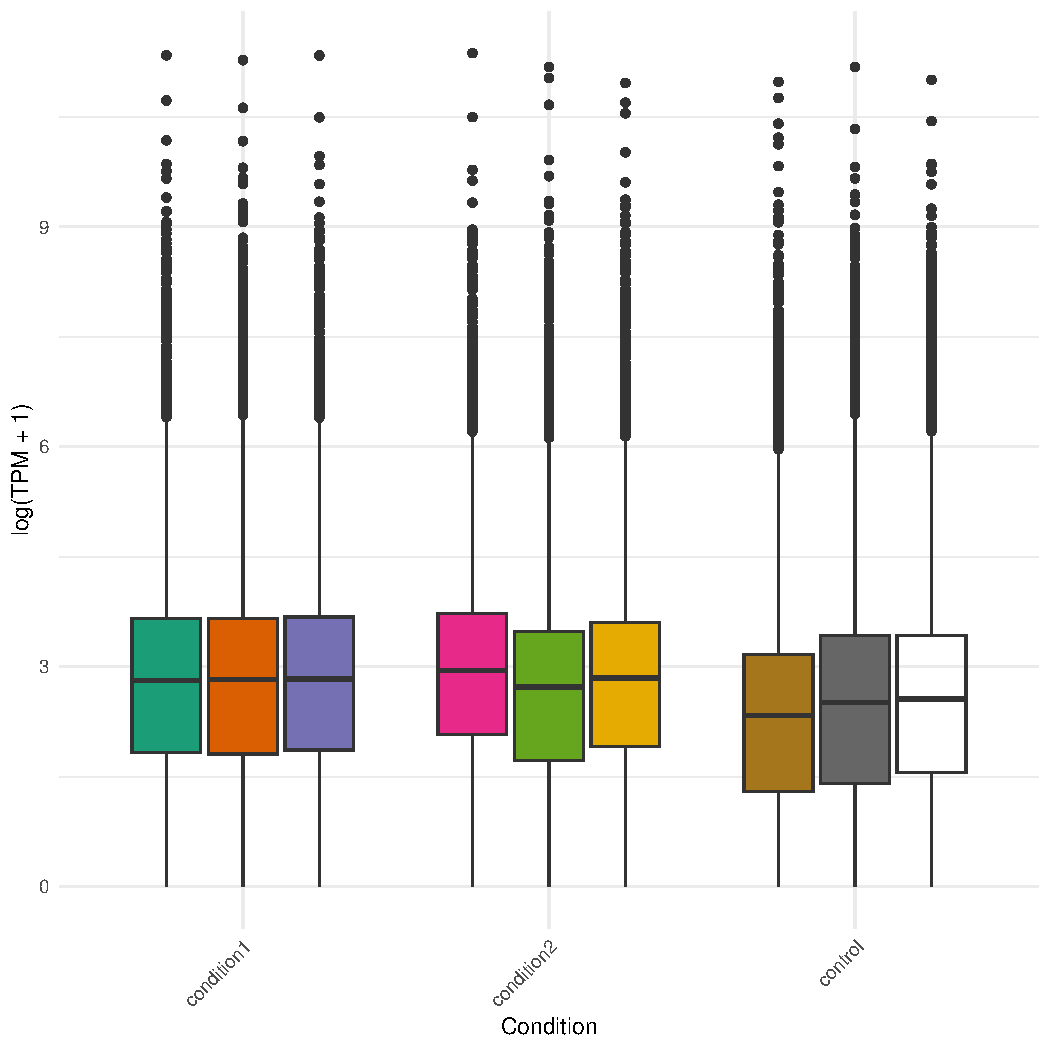
\includegraphics[width=0.8\textwidth]{6_3_kallisto_boxplot.pdf}
  \caption{Box plots of the TPM values for the Kallisto analysis}\label{fig:box_kallisto}
\end{figure}

The correlation between the technical and biological replicates of the Kallisto 
alignment was calculated and visualized in 
figure~\ref{fig:corr_kallisto}.
The samples of condition 1 showed a high correlation between each other. The replicates for 
the control condition as well as for condition 2 differed more in comparison. 

\begin{figure}[H]
  \center
  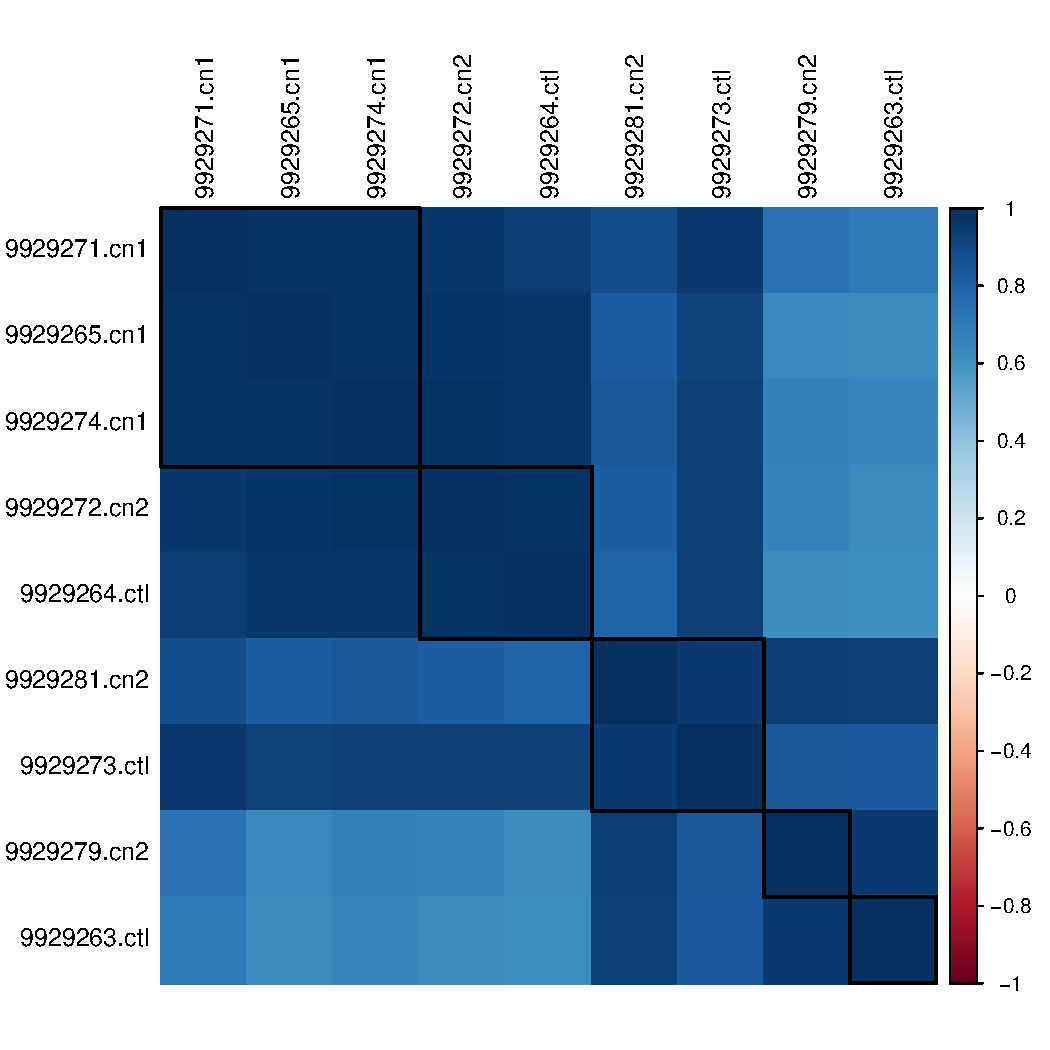
\includegraphics[width=0.7\textwidth]{6_3_kallisto_corr_matrix.pdf}
  \caption{Correlation plot for the technical and biological replicates of the Kallisto
  analysis}\label{fig:corr_kallisto}
\end{figure}

\subsection{Bowtie2}

For the Bowtie2 alignment we analysed how many reads were mapped once, multiple times or were 
not aligned at all. All replicates showed similar ratios. 
The mapping of the reads of Bowtie2 is shown in figure~\ref{fig:bar_bowtie}

\begin{figure}[H]
  \center
  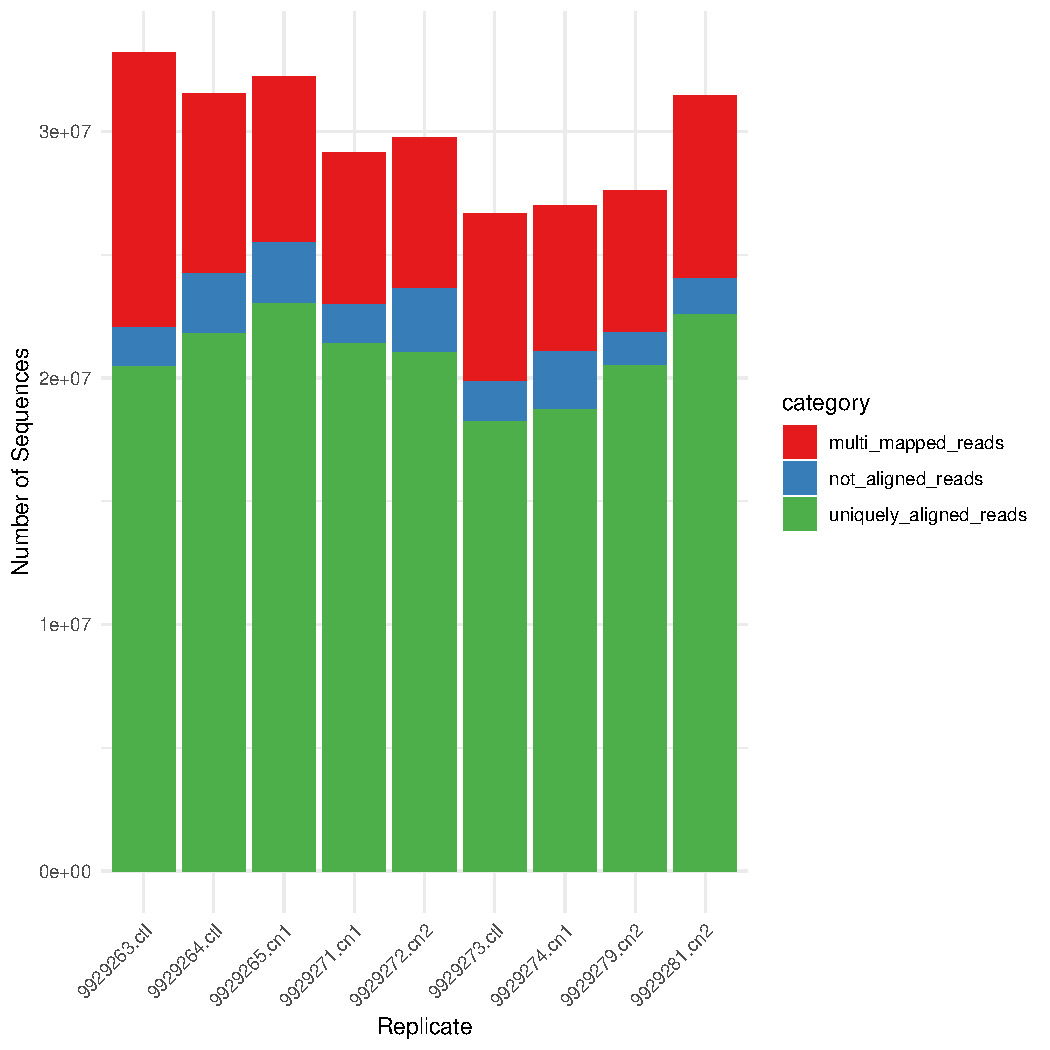
\includegraphics[width=0.7\textwidth]{6_3_bowtie_alignment_bar.pdf}
  \caption{Mapping of the reads of the Bowtie2 alignment}\label{fig:bar_bowtie}
\end{figure}

\subsection{Comparison Kallisto and Bowtie2}
The distribution of the TPM values obtained by Kallisto and Bowtie2 were similar. 
The Bowtie2 results also showed slightly lower median for the control group.
For both programs and for both conditions the log fold changes have been calculated 
and the distribution was plotted in figure~\ref{fig:dist_lfc}.
The distribution of TPM values looks comparable between the programs. S shift to the positive 
log fold changes can be seen. 

\begin{figure}[H]
  \center
  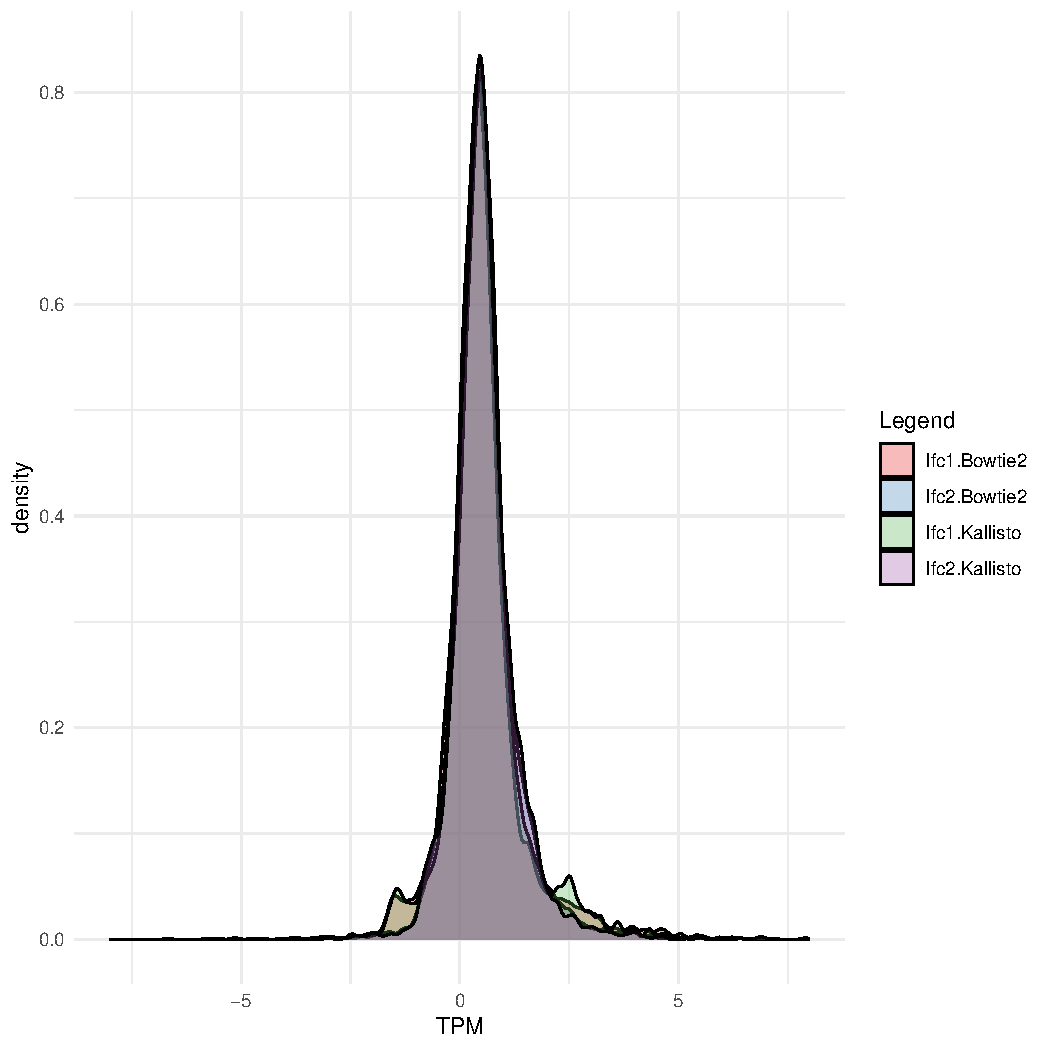
\includegraphics[width=0.7\textwidth]{6_post_all_lfc_density.pdf}
  \caption{Grouped box plots of the three biological replicates per group}\label{fig:dist_lfc}
\end{figure}

\section{Weighted Gene Co-expression Network Analysis}

The word cloud generated for the genes in the significant module is shown in figure~\ref{fig:worcloud_wgcna}

\begin{figure}[H]
  \center
  
\includegraphics[width=0.7\textwidth]{10_6_wordcloud_me2.pdf}
  \caption{Word Cloud for the Module Eigengen 2}\label{fig:worcloud_wgcna}
\end{figure}

\section{Differential Gene Expression}

\begin{figure}[H]
    \centering
    \begin{subfigure}[b]{0.45\textwidth} 
        \centering
        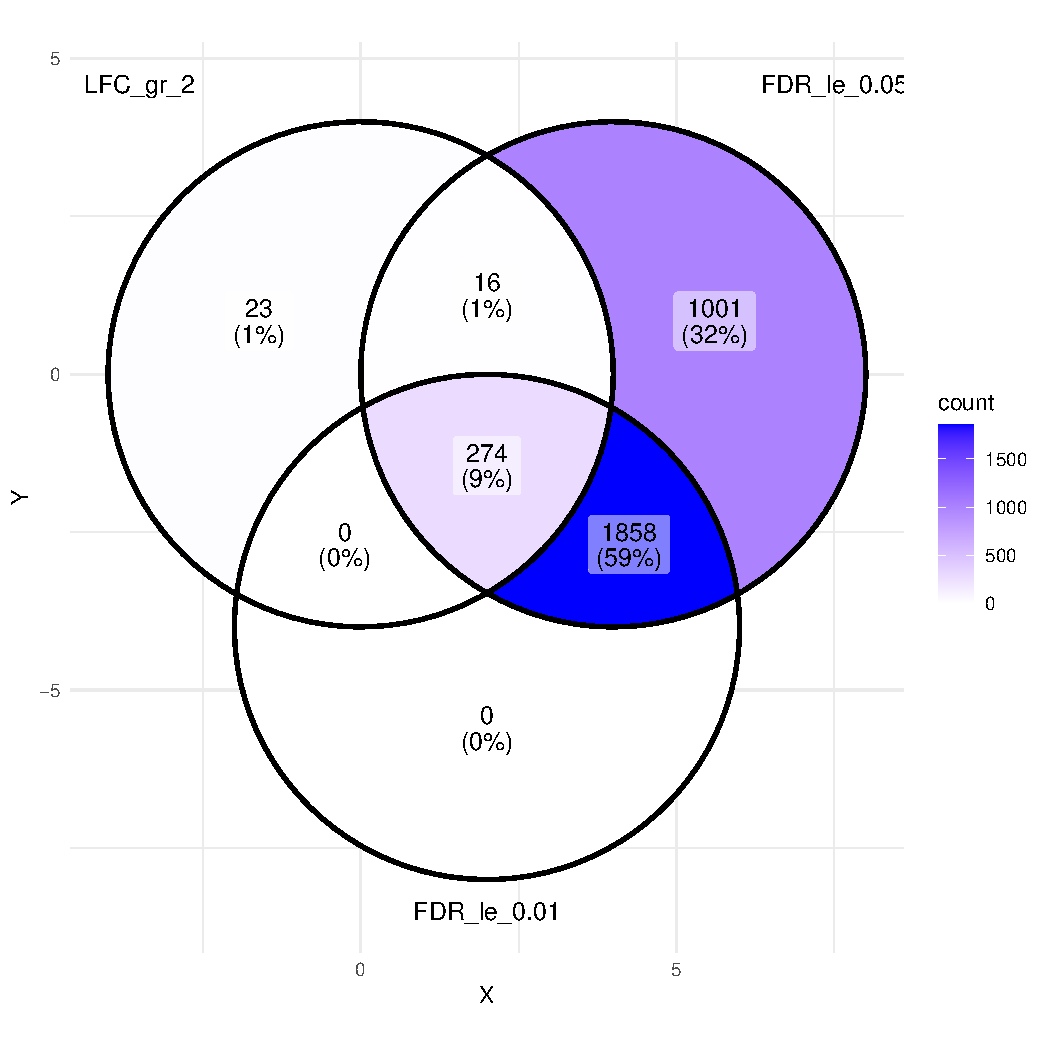
\includegraphics[width=\textwidth]{11_edgeR_venn_diagram_cn1.pdf} 
        \caption{}
        \label{fig:venn_edgeR_1}
    \end{subfigure}
    \hfill % Horizontal space between subfigures
    % Second subfigure
    \begin{subfigure}[b]{0.45\textwidth} % Adjust width as needed
        \centering
        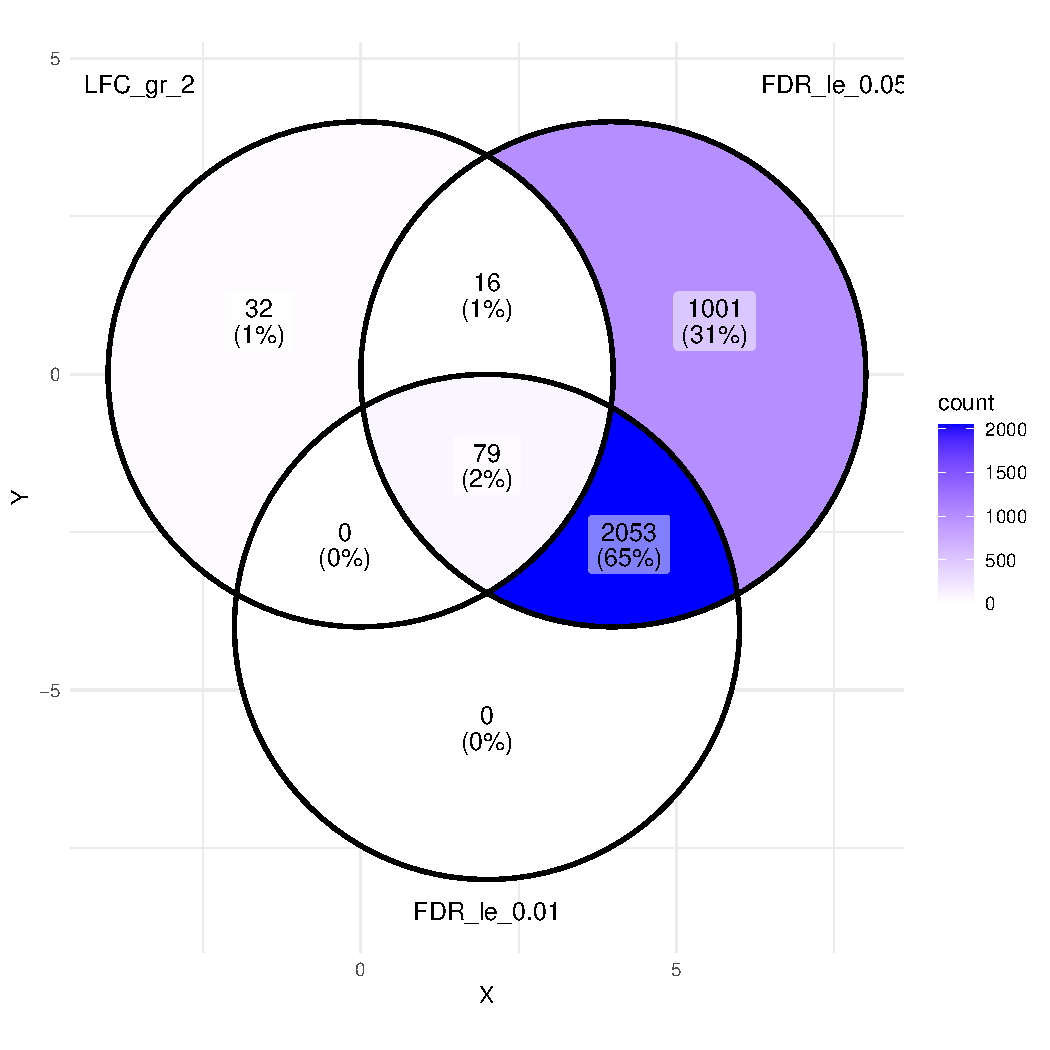
\includegraphics[width=\textwidth]{11_edgeR_venn_diagram_cn2.pdf} % Replace with your image
        \caption{}
        \label{fig:venn_edgeR_2}
    \end{subfigure}
    \caption{Caption for the entire figure.}
    \label{fig:venn_edgeR}
\end{figure}

\begin{figure}[H]
    \centering
    \begin{subfigure}[b]{0.45\textwidth} 
        \centering
        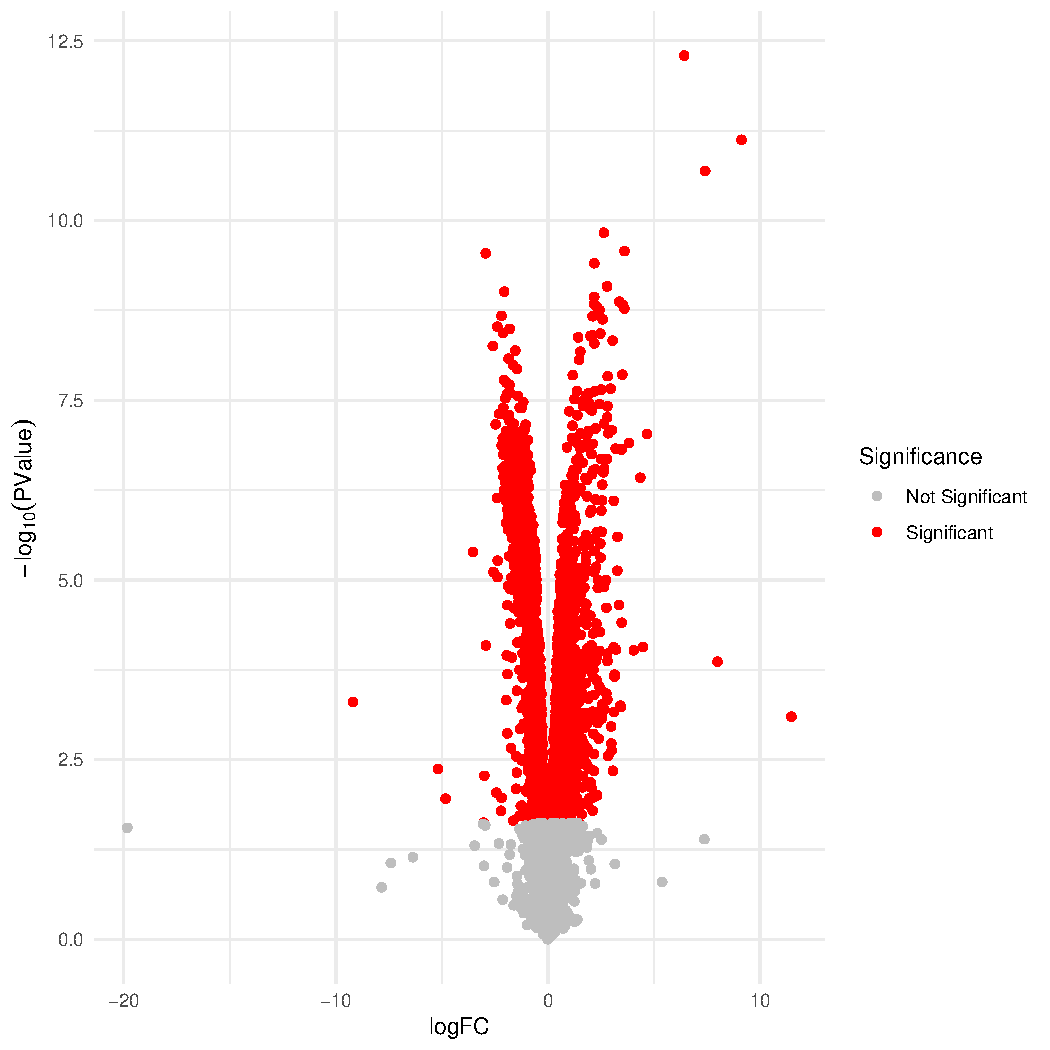
\includegraphics[width=\textwidth]{11_edgeR_volcano_con1.pdf} 
        \caption{}
        \label{fig:vol_edgeR_1}
    \end{subfigure}
    \hfill % Horizontal space between subfigures
    % Second subfigure
    \begin{subfigure}[b]{0.45\textwidth} % Adjust width as needed
        \centering
        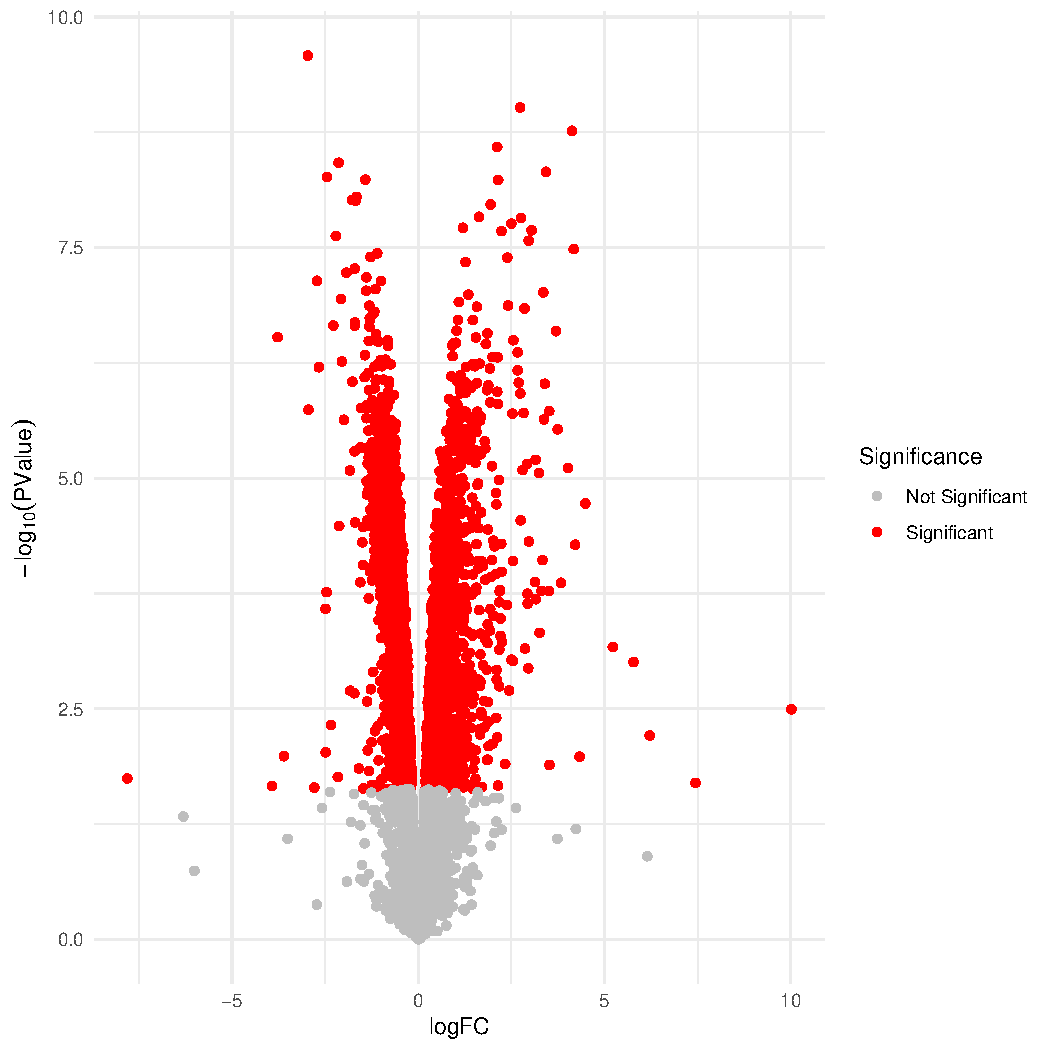
\includegraphics[width=\textwidth]{11_edgeR_volcano_con2.pdf} % Replace with your image
        \caption{}
        \label{fig:vol_edgeR_2}
    \end{subfigure}
    \caption{Caption for the entire figure.}
    \label{fig:vol_edgeR}
\end{figure}

\begin{figure}[H]
  \center
  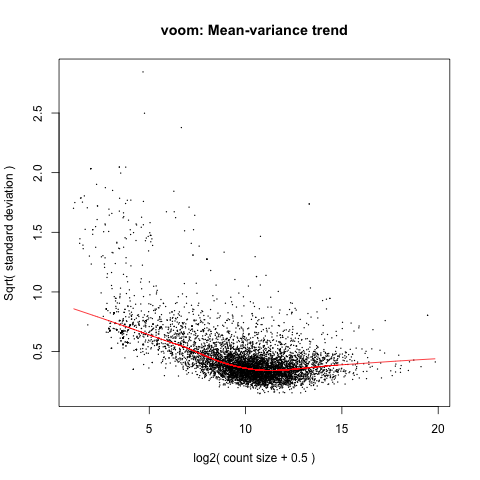
\includegraphics[width=0.7\textwidth]{11_voom_plot1.png}
  \caption{Voom plot}\label{fig:voom}
\end{figure}


\begin{figure}[H]
    \centering
    \begin{subfigure}[b]{0.45\textwidth} 
        \centering
        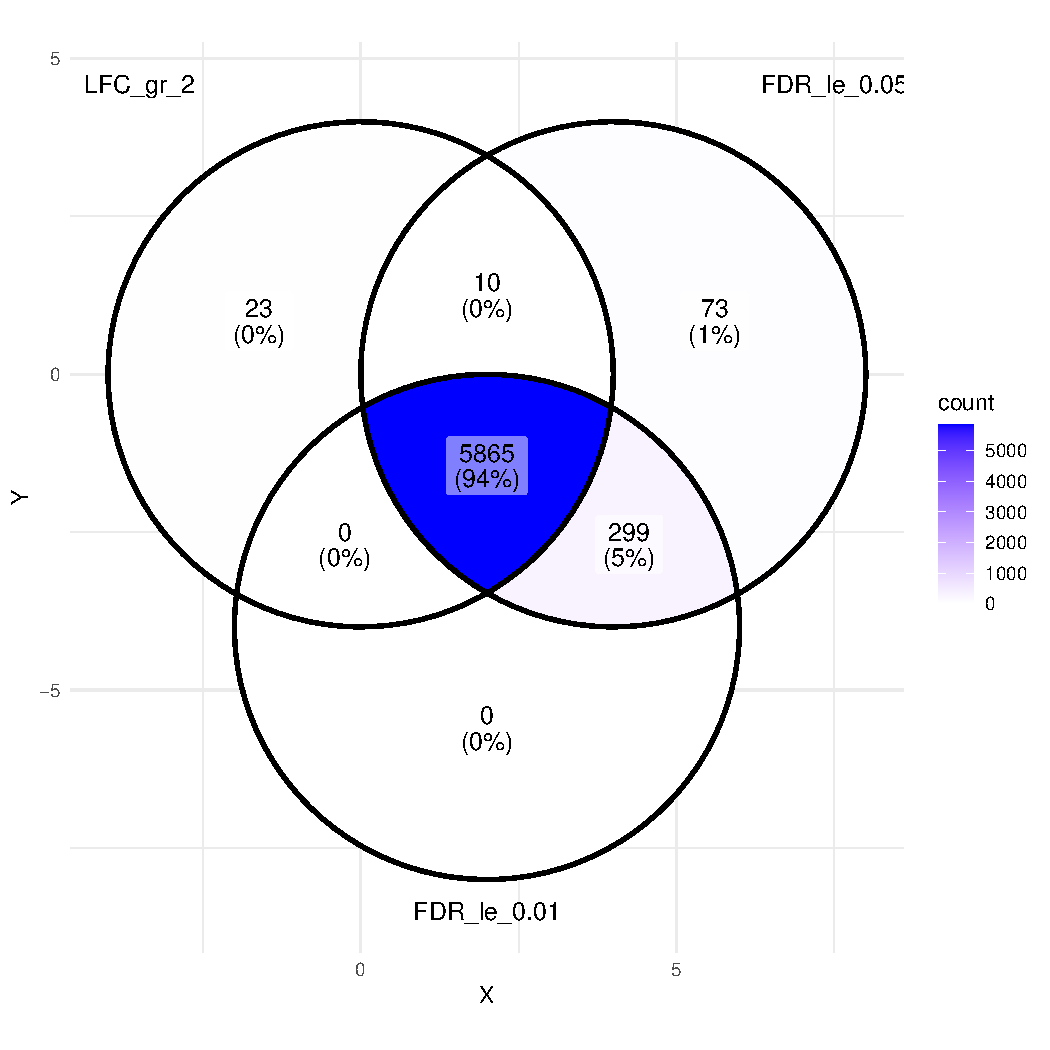
\includegraphics[width=\textwidth]{11_limma_venn_diagram_cn1.pdf} 
        \caption{}
        \label{fig:venn_limma_1}
    \end{subfigure}
    \hfill % Horizontal space between subfigures
    % Second subfigure
    \begin{subfigure}[b]{0.45\textwidth} % Adjust width as needed
        \centering
        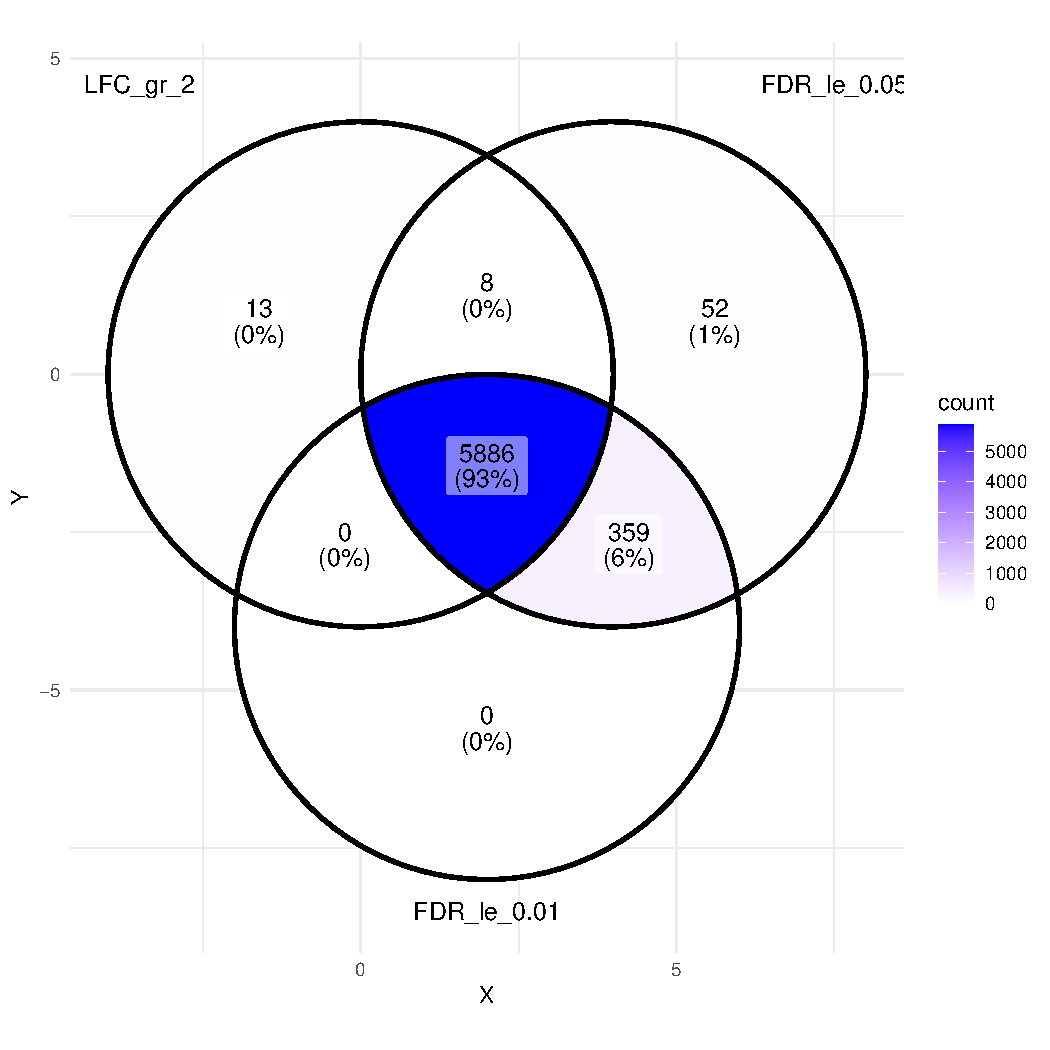
\includegraphics[width=\textwidth]{11_limma_venn_diagram_cn2.pdf} % Replace with your image
        \caption{}
        \label{fig:venn_limma_2}
    \end{subfigure}
    \caption{Caption for the entire figure.}
    \label{fig:venn_limma}
\end{figure}

\begin{figure}[H]
    \centering
    \begin{subfigure}[b]{0.45\textwidth} 
        \centering
        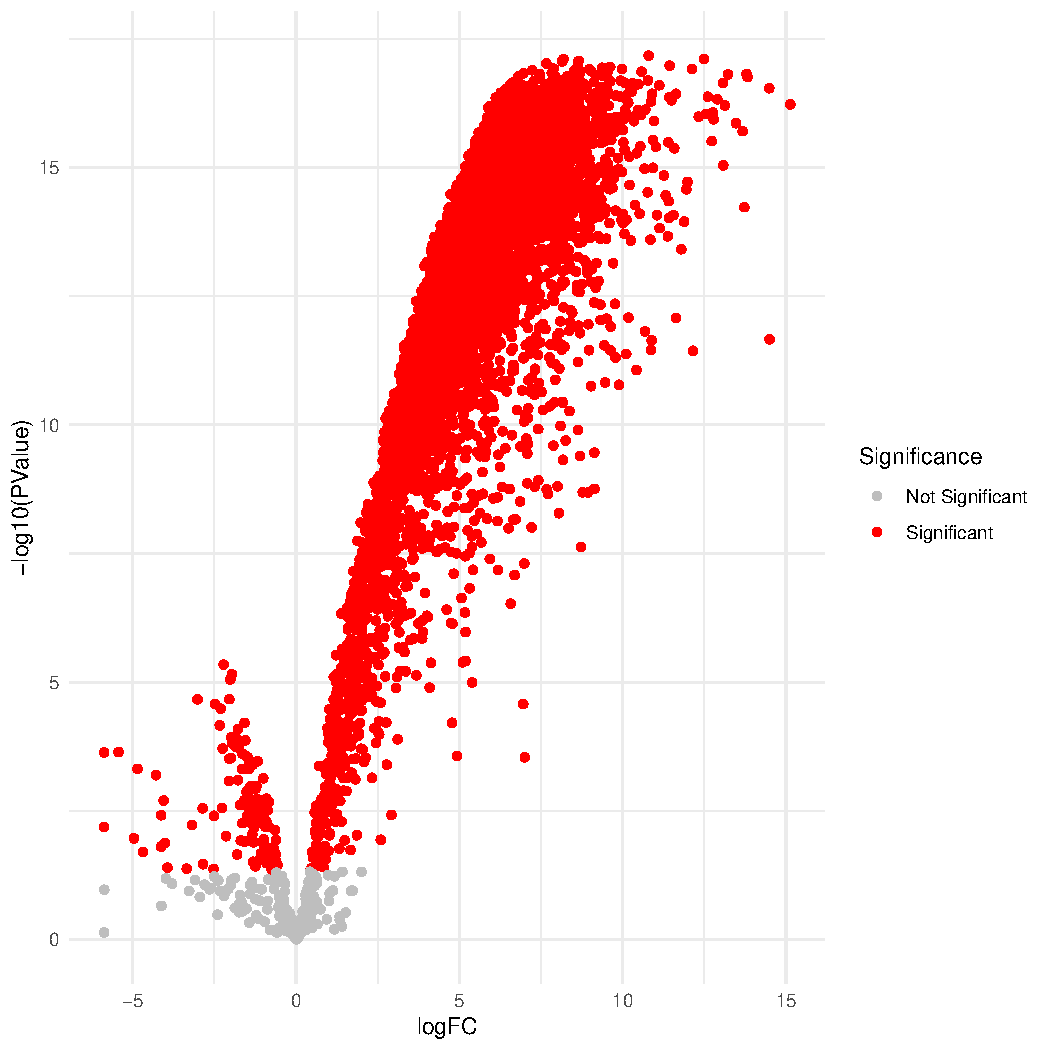
\includegraphics[width=\textwidth]{11_limma_volcano_con1.pdf} 
        \caption{}
        \label{fig:vol_limma_1}
    \end{subfigure}
    \hfill % Horizontal space between subfigures
    % Second subfigure
    \begin{subfigure}[b]{0.45\textwidth} % Adjust width as needed
        \centering
        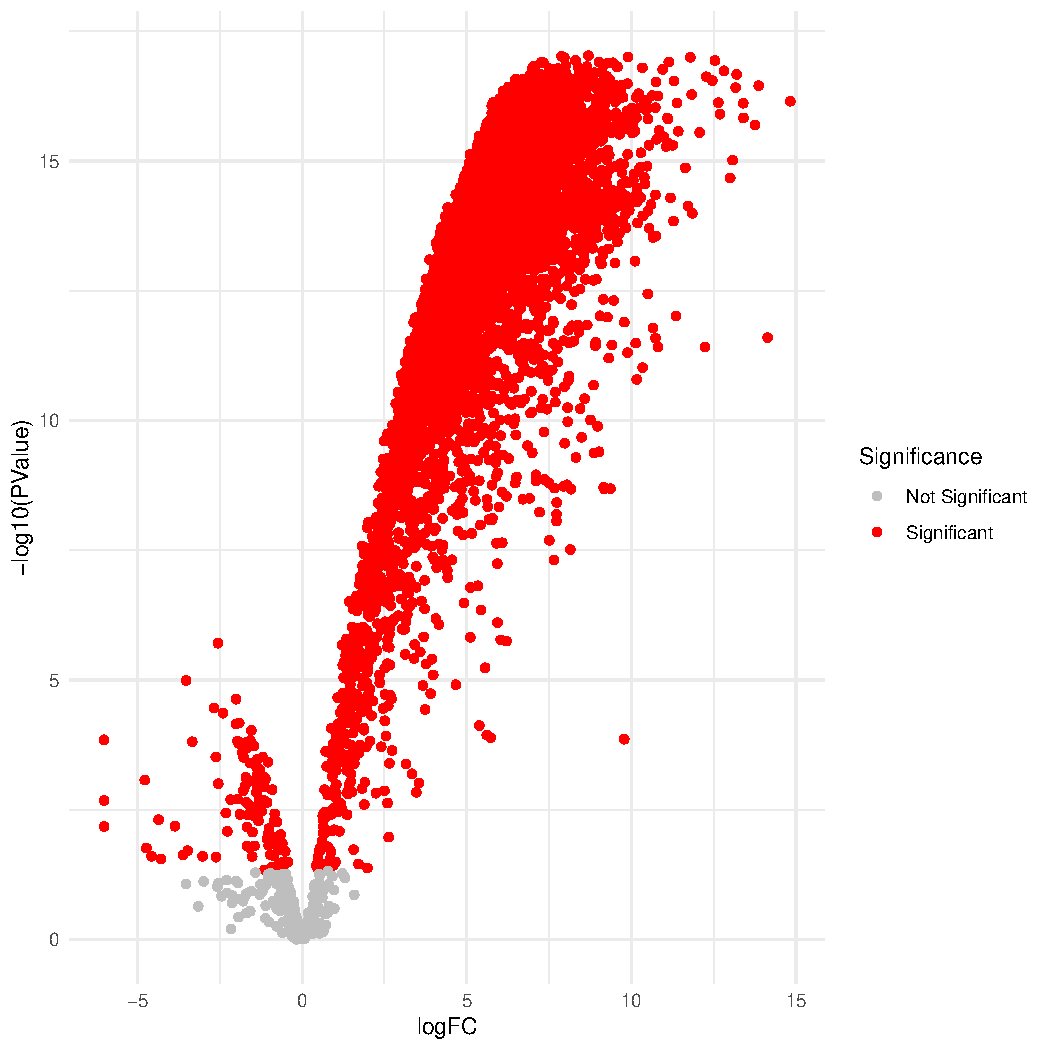
\includegraphics[width=\textwidth]{11_limma_volcano_con2.pdf} % Replace with your image
        \caption{}
        \label{fig:vol_limma_2}
    \end{subfigure}
    \caption{Caption for the entire figure.}
    \label{fig:vol_limma}
\end{figure}

\begin{figure}[H]
    \centering
    % Top-left subfigure
    \begin{subfigure}[b]{0.45\textwidth}
        \centering
        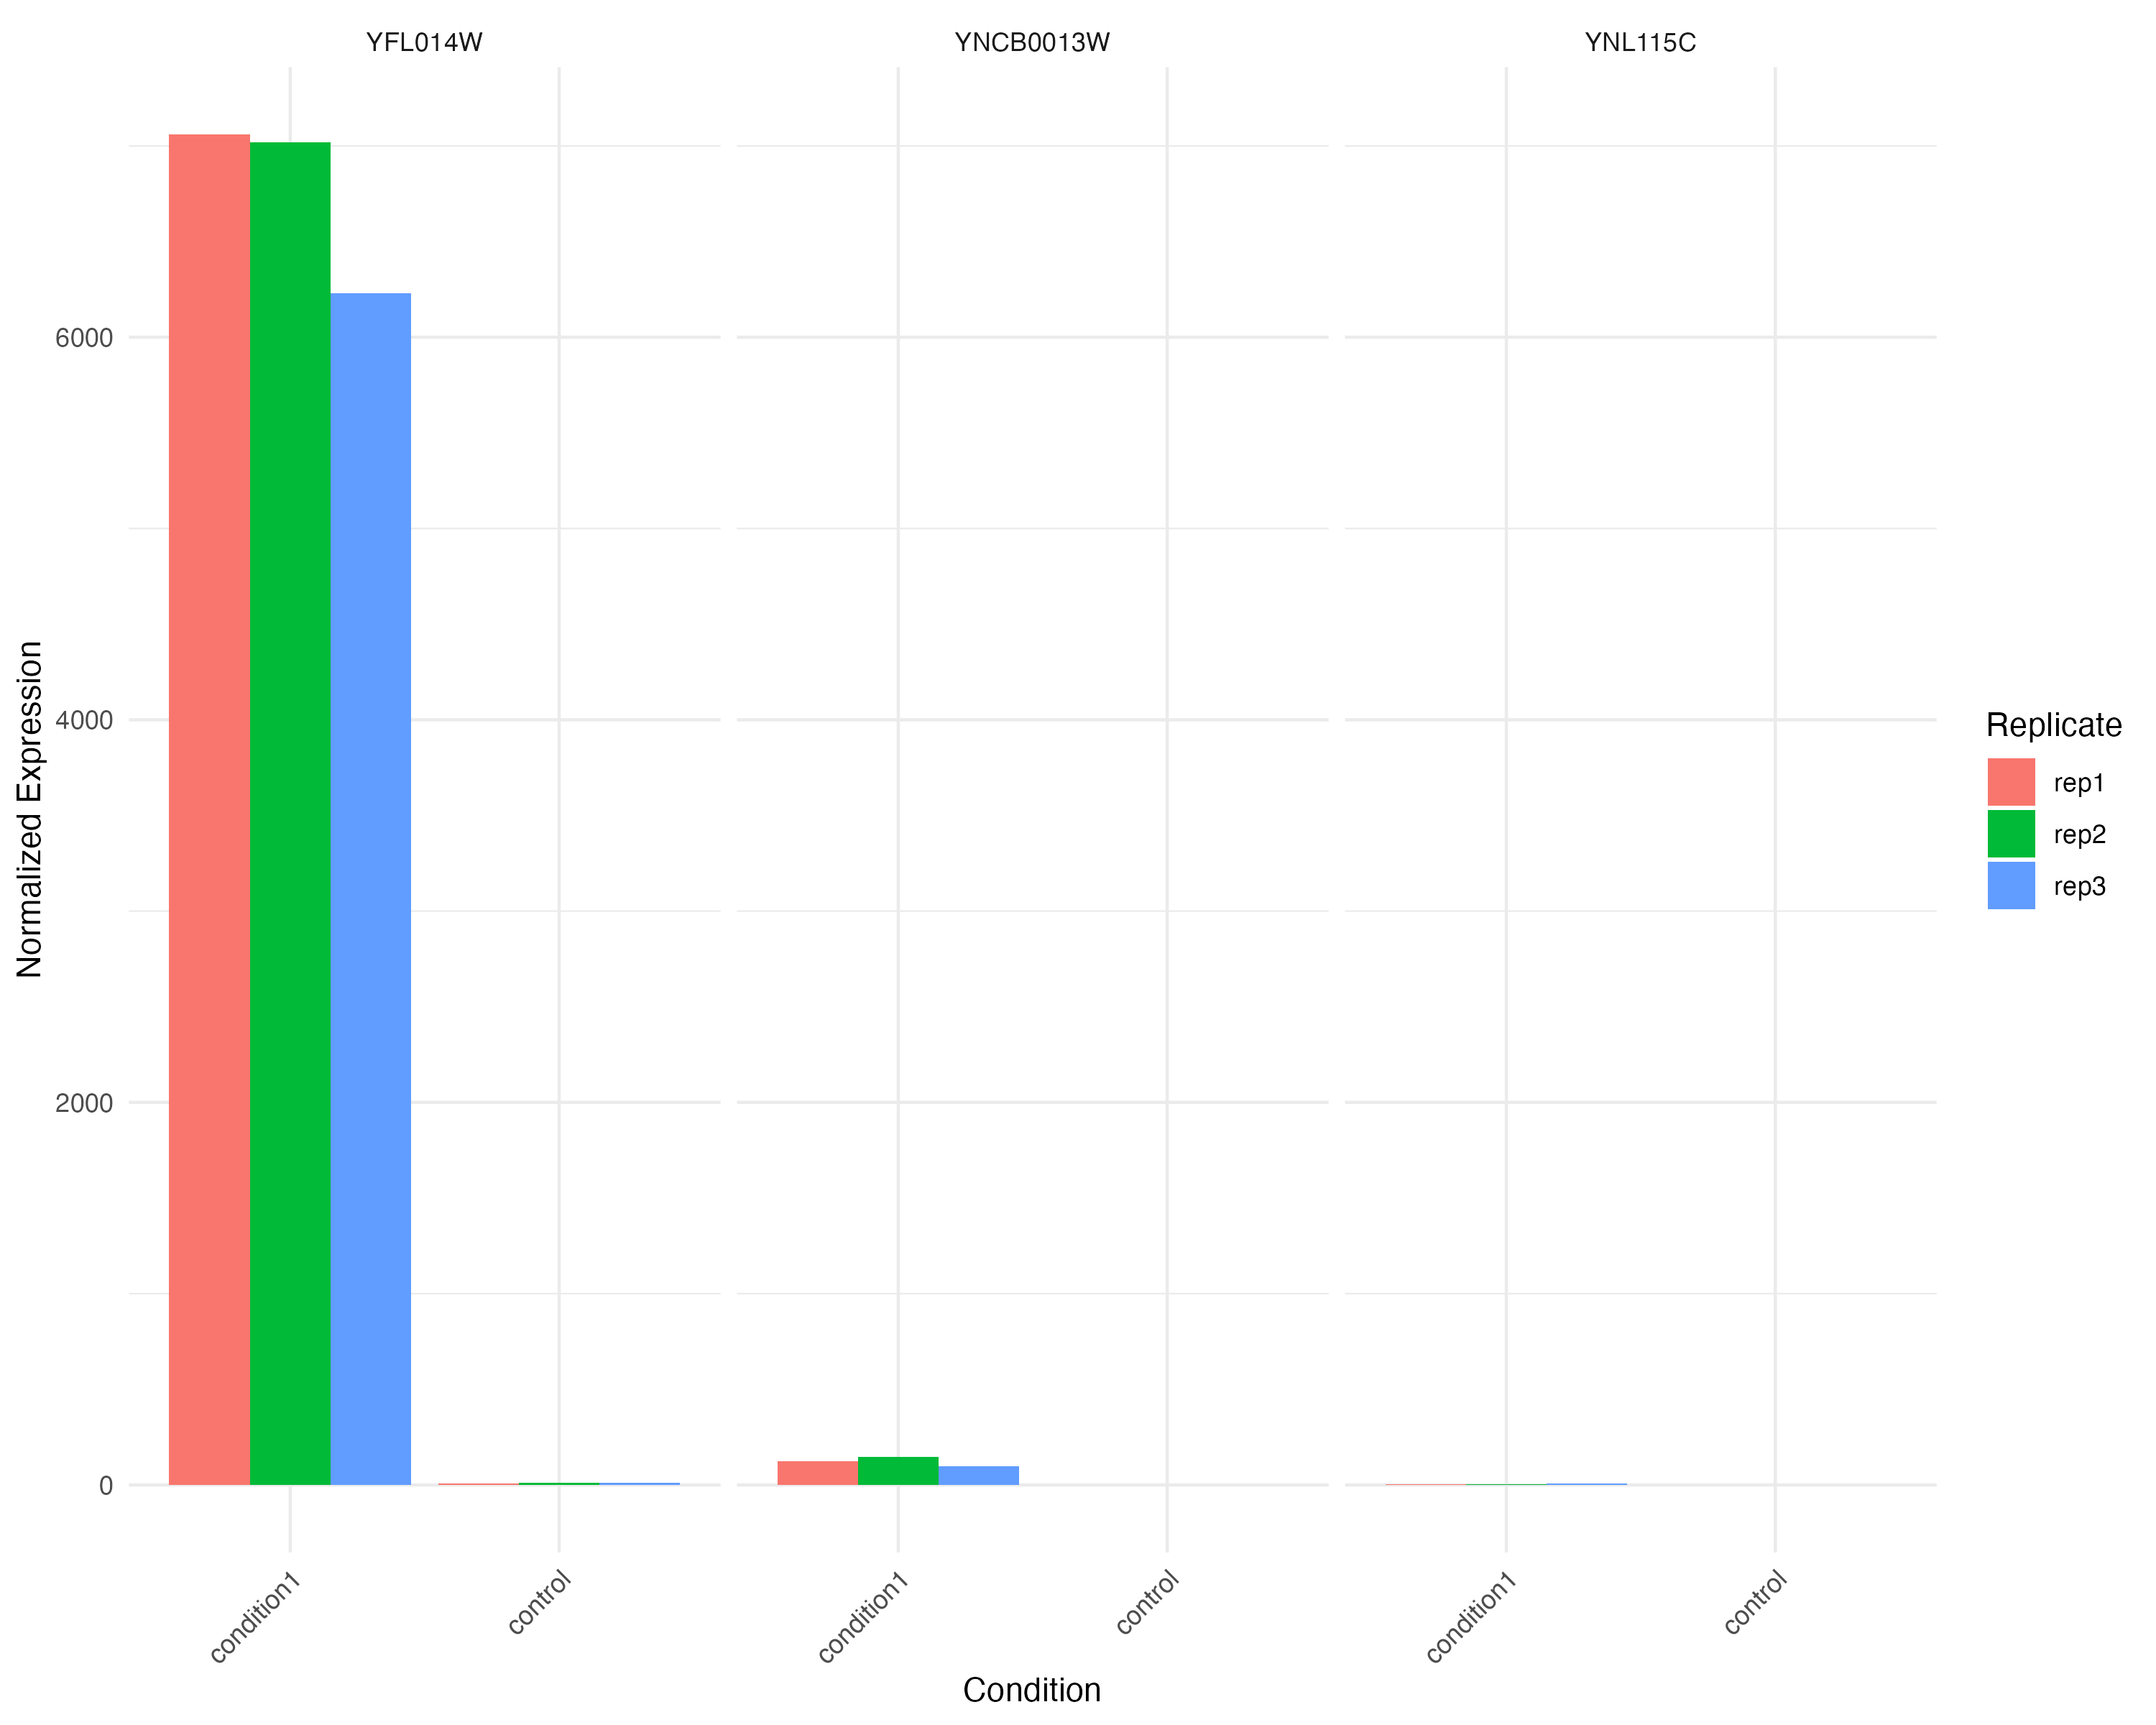
\includegraphics[width=\textwidth]{11_edgeR_top_positive_genes_expression_by_condition1.png} % Replace with your image
        \caption{}
        \label{fig:pos_edger_1}
    \end{subfigure}
    \hfill
    % Top-right subfigure
    \begin{subfigure}[b]{0.45\textwidth}
        \centering
        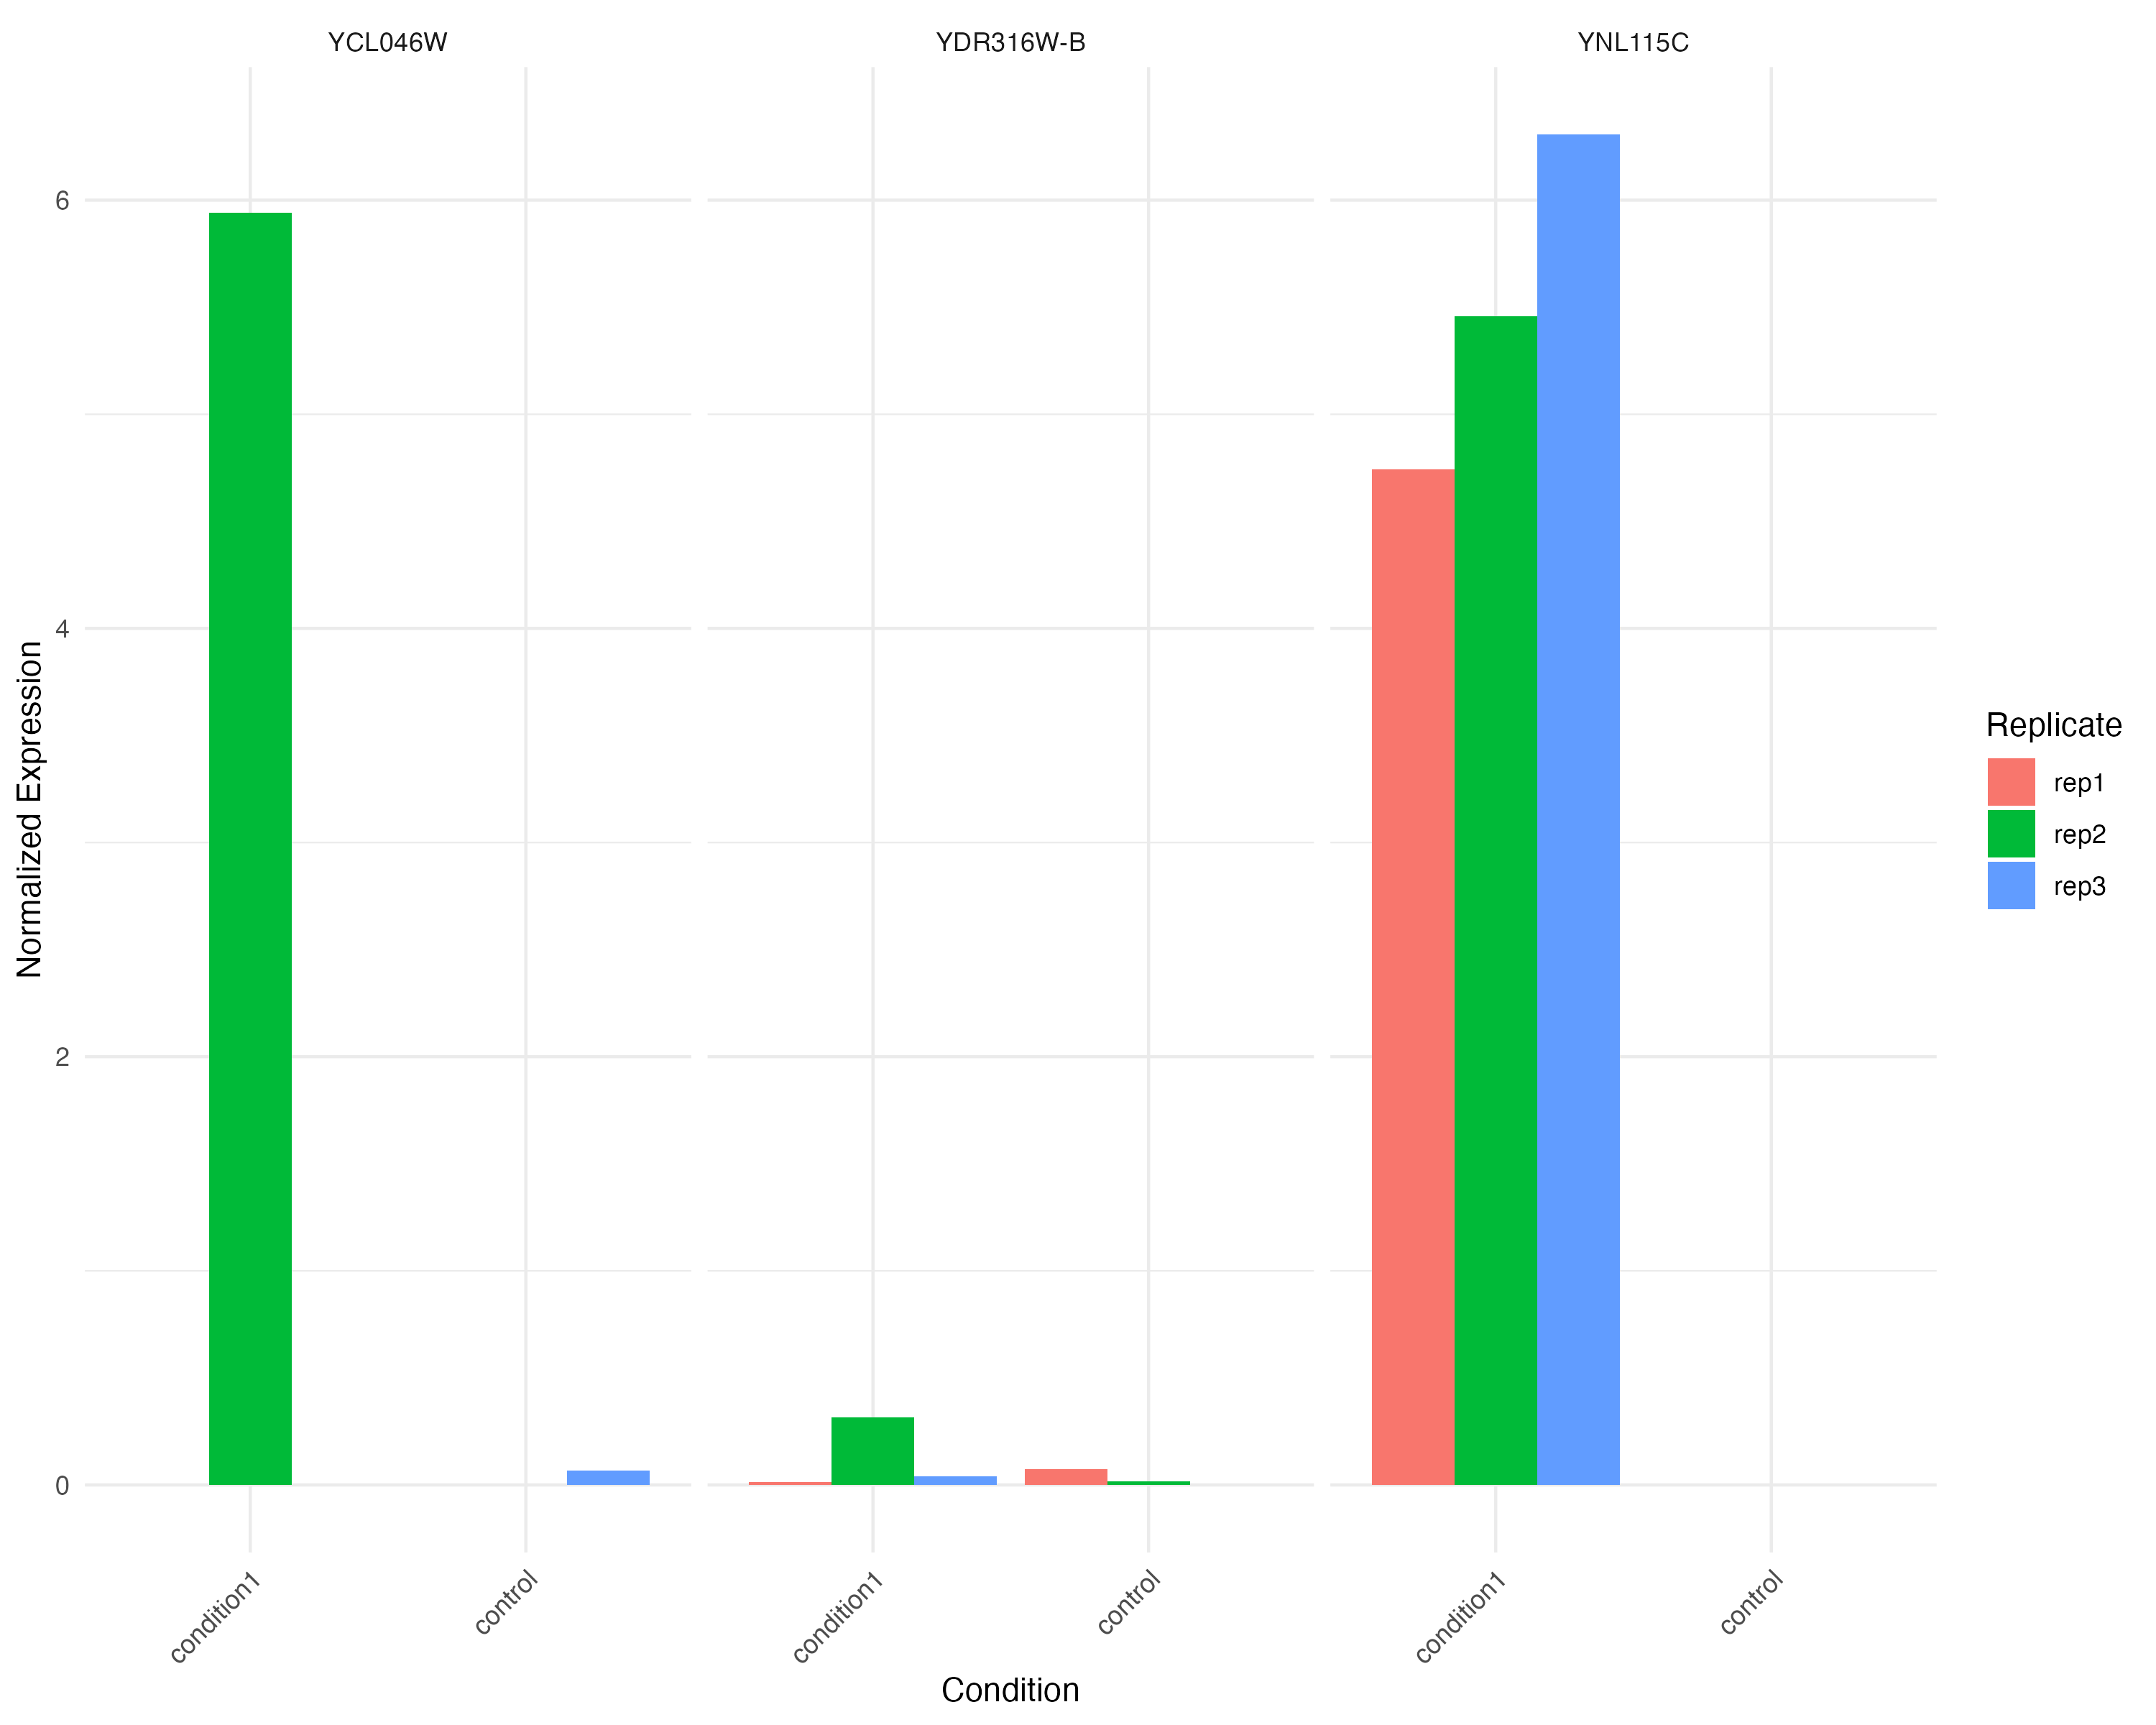
\includegraphics[width=\textwidth]{11_edgeR_top_positive_genes_expression_by_condition2.png} % Replace with your image
        \caption{}
        \label{fig:pos_edger_2}
    \end{subfigure}
    \vskip\baselineskip % Vertical space between rows
    % Bottom-left subfigure
    \begin{subfigure}[b]{0.45\textwidth}
        \centering
        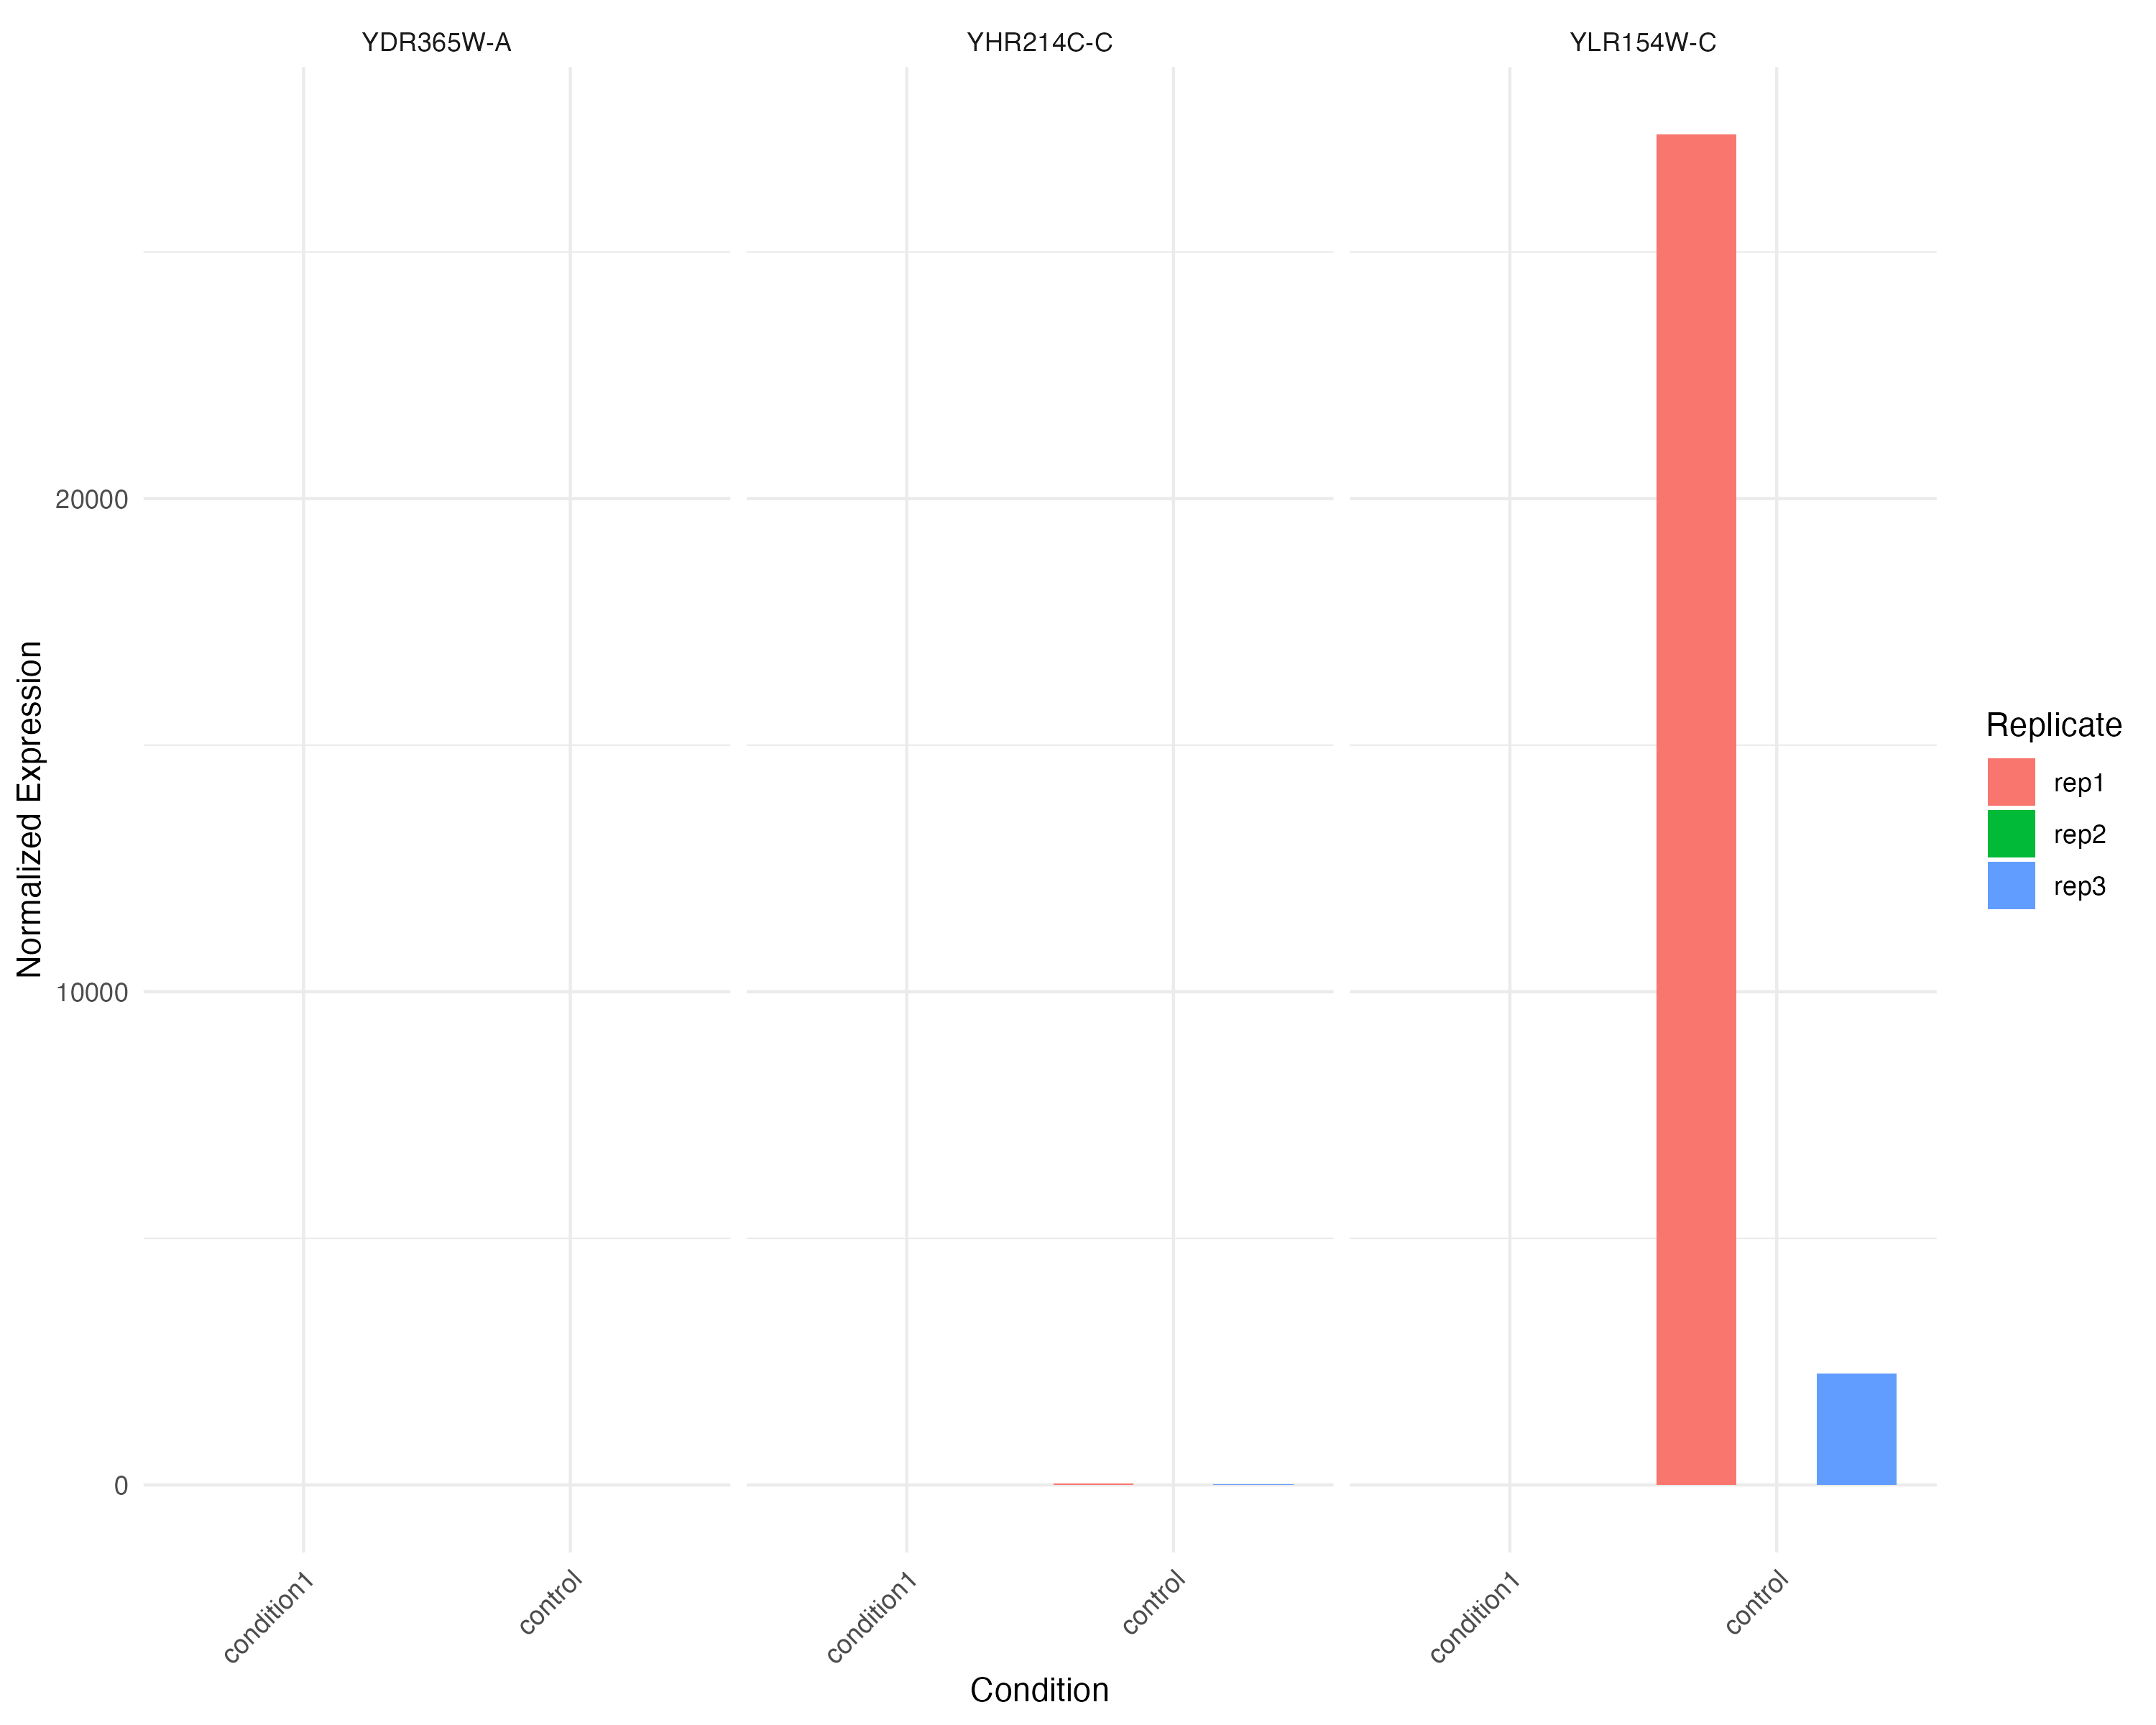
\includegraphics[width=\textwidth]{11_edgeR_top_negative_genes_expression_by_condition1.png} % Replace with your image
        \caption{}
        \label{fig:neg_edger_1}
    \end{subfigure}
    \hfill
    % Bottom-right subfigure
    \begin{subfigure}[b]{0.45\textwidth}
        \centering
        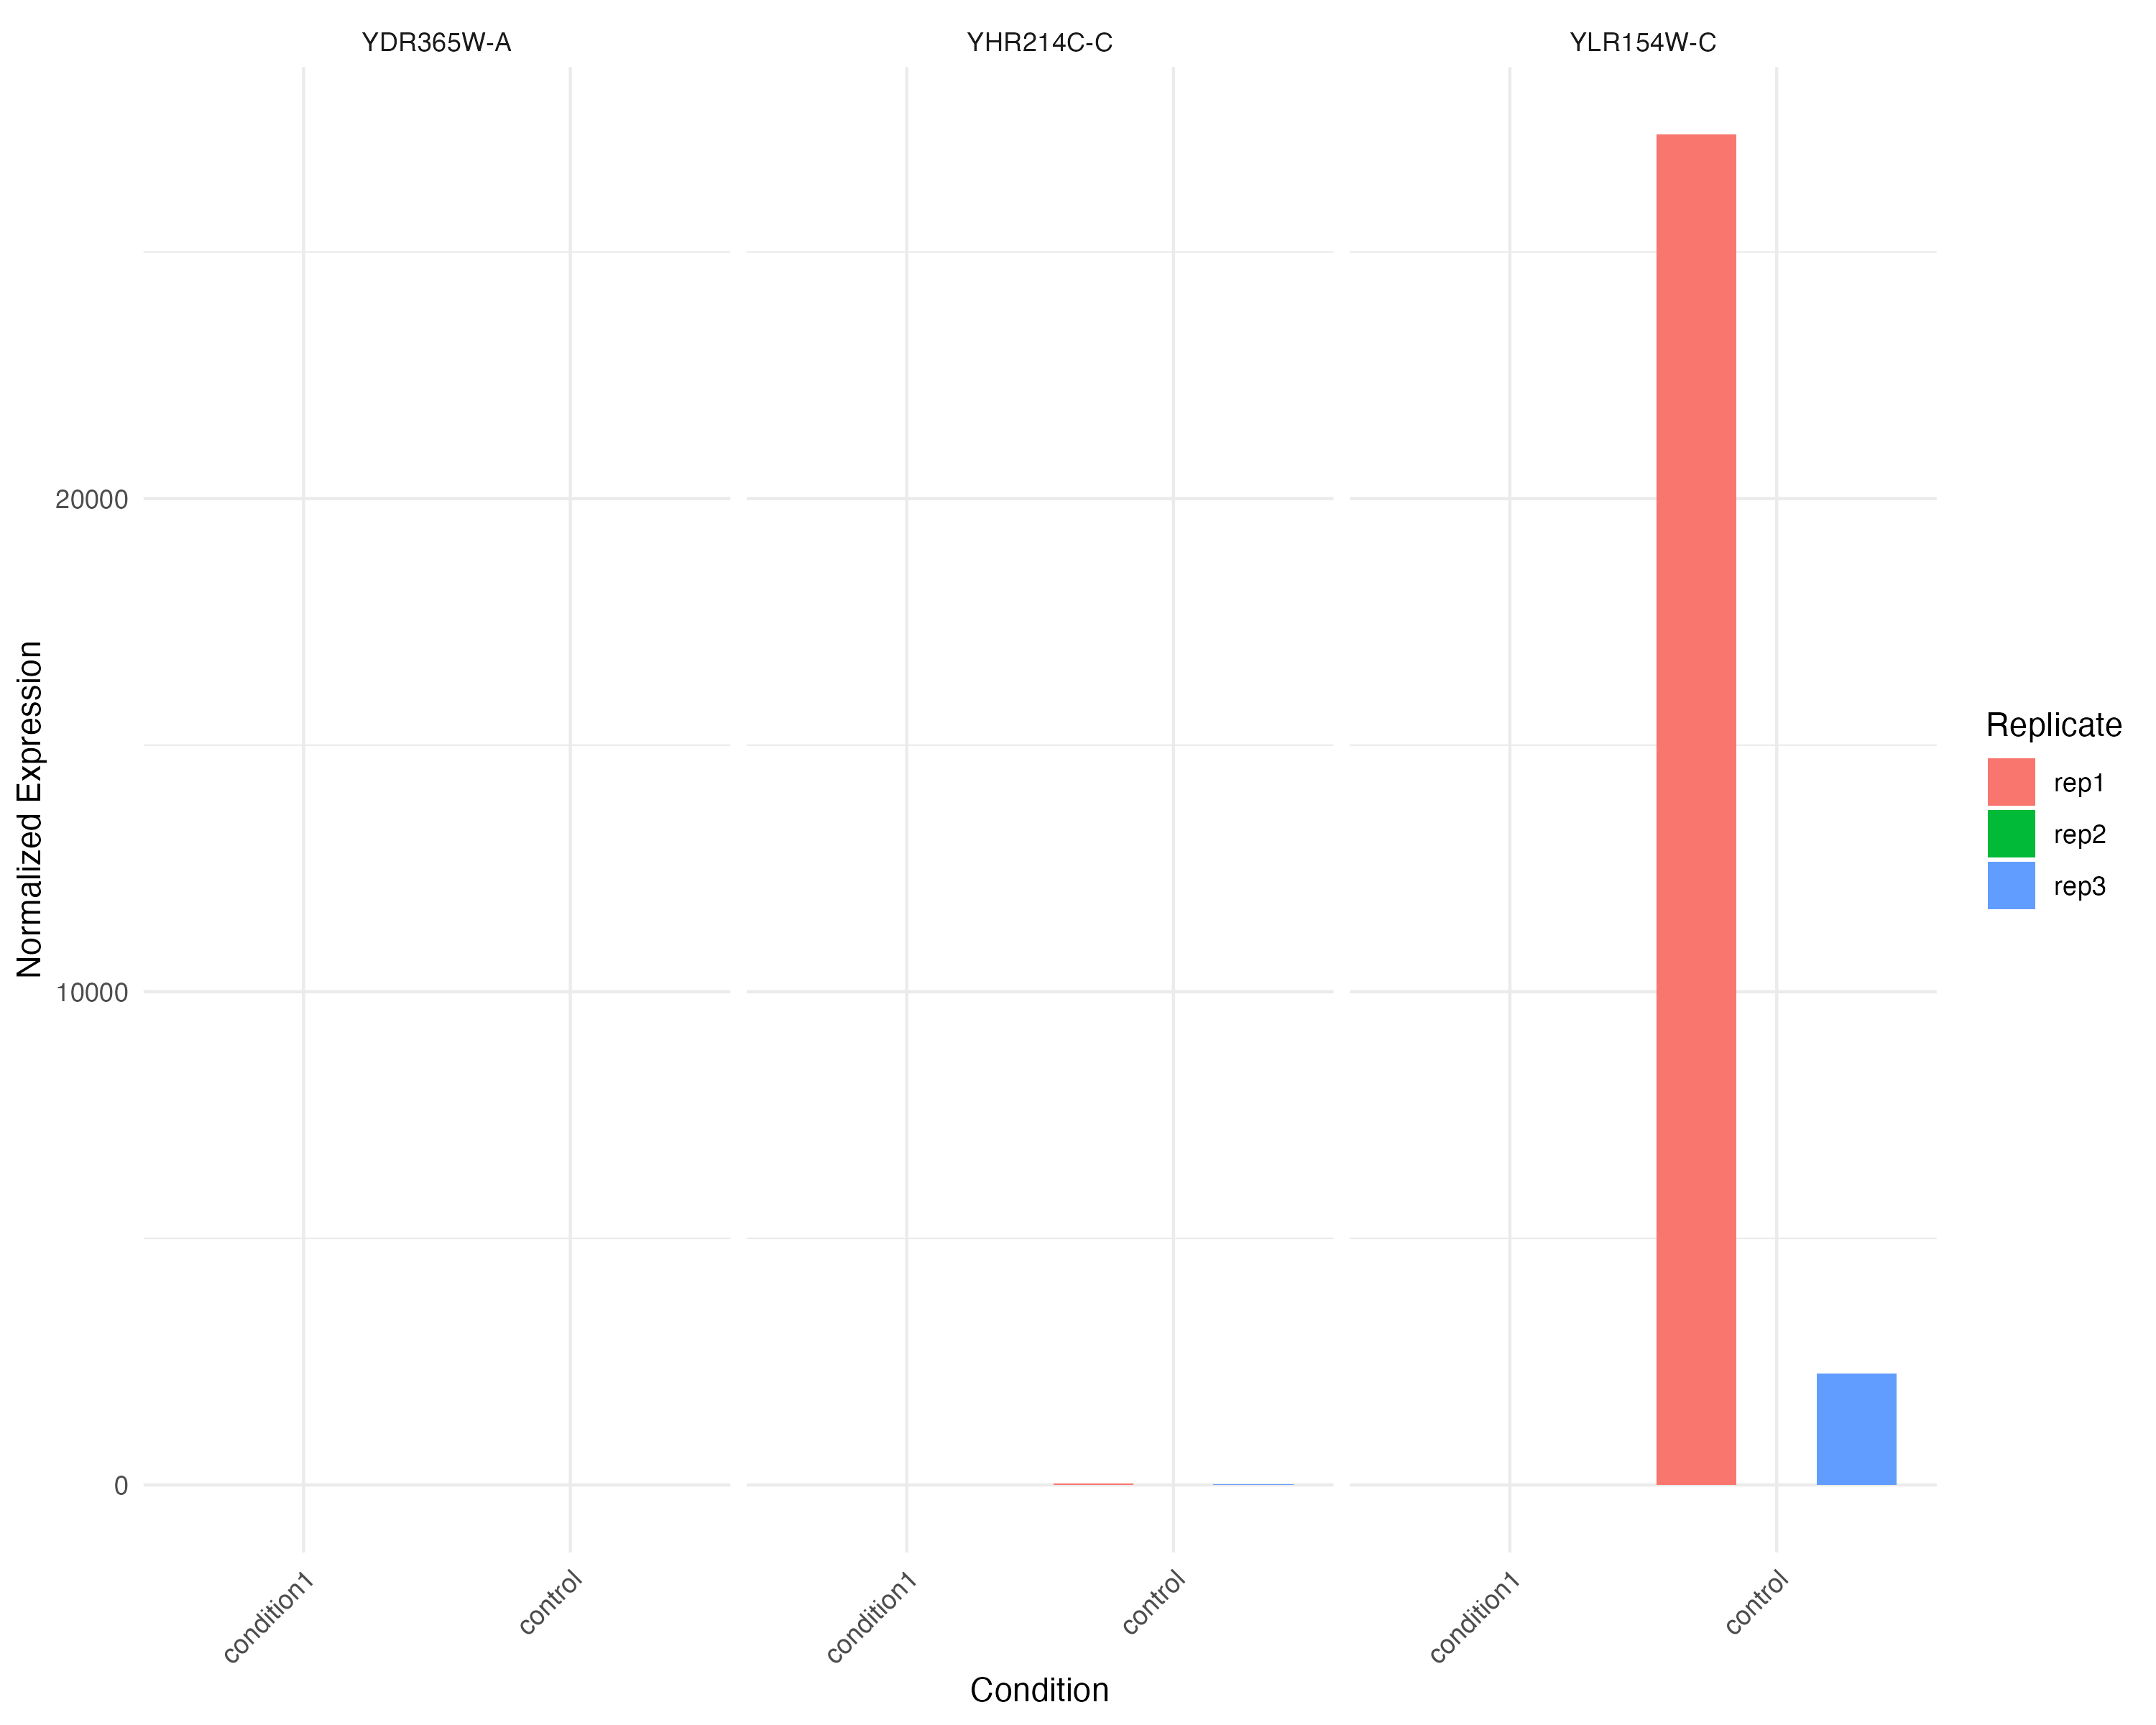
\includegraphics[width=\textwidth]{11_edgeR_top_negative_genes_expression_by_condition1.png} % Replace with your image
        \caption{}
        \label{fig:neg_edger_2}
    \end{subfigure}
    % Overall figure caption
    \caption{Results from the four experiments: (a) First experiment, (b) Second experiment, (c) Third experiment, (d) Fourth experiment.}
    \label{fig:top_edger}
\end{figure}

\begin{figure}[H]
    \centering
    % Top-left subfigure
    \begin{subfigure}[b]{0.45\textwidth}
        \centering
        
\includegraphics[width=\textwidth]{11_edgeR_wordcloud_cn1_up.pdf} % Replace with your image
        \caption{}
        \label{fig:wc_pos_edger_1}
    \end{subfigure}
    \hfill
    % Top-right subfigure
    \begin{subfigure}[b]{0.45\textwidth}
        \centering
        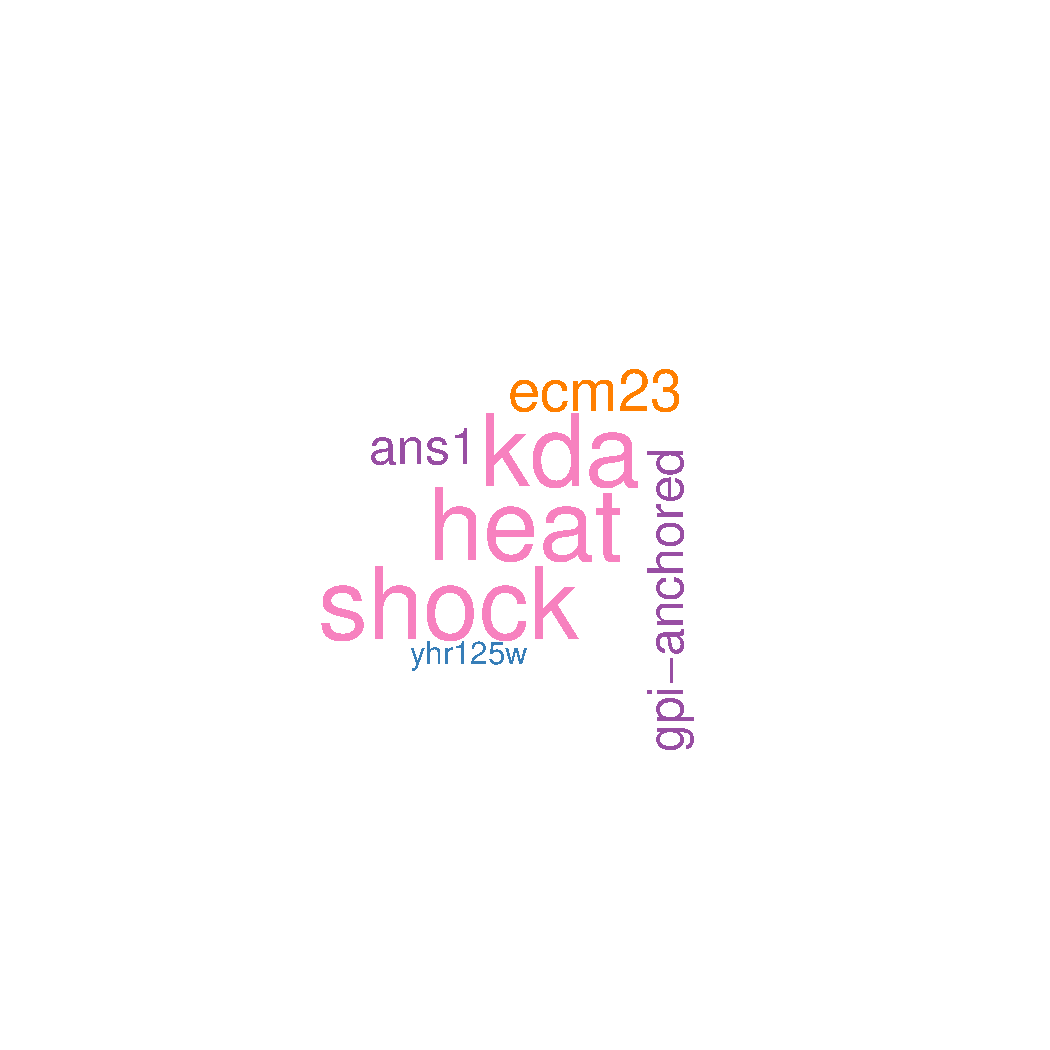
\includegraphics[width=\textwidth]{11_edgeR_wordcloud_cn2_up.pdf} % Replace with your image
        \caption{}
        \label{fig:wc_pos_edger_2}
    \end{subfigure}
    \vskip\baselineskip % Vertical space between rows
    % Bottom-left subfigure
    \begin{subfigure}[b]{0.45\textwidth}
        \centering
        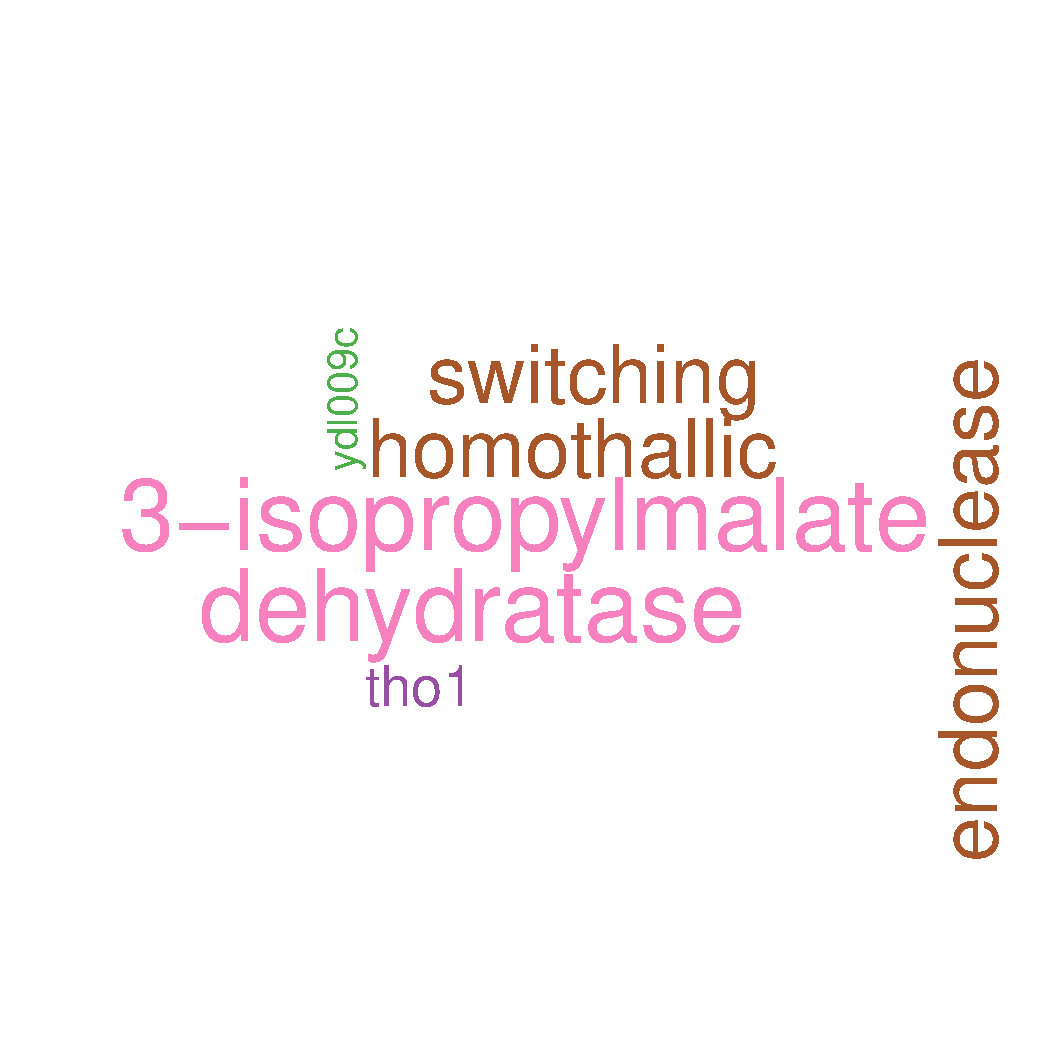
\includegraphics[width=\textwidth]{11_edgeR_wordcloud_cn1_down.pdf} % Replace with your image
        \caption{}
        \label{fig:wc_neg_edger_1}
    \end{subfigure}
    \hfill
    % Bottom-right subfigure
    \begin{subfigure}[b]{0.45\textwidth}
        \centering
        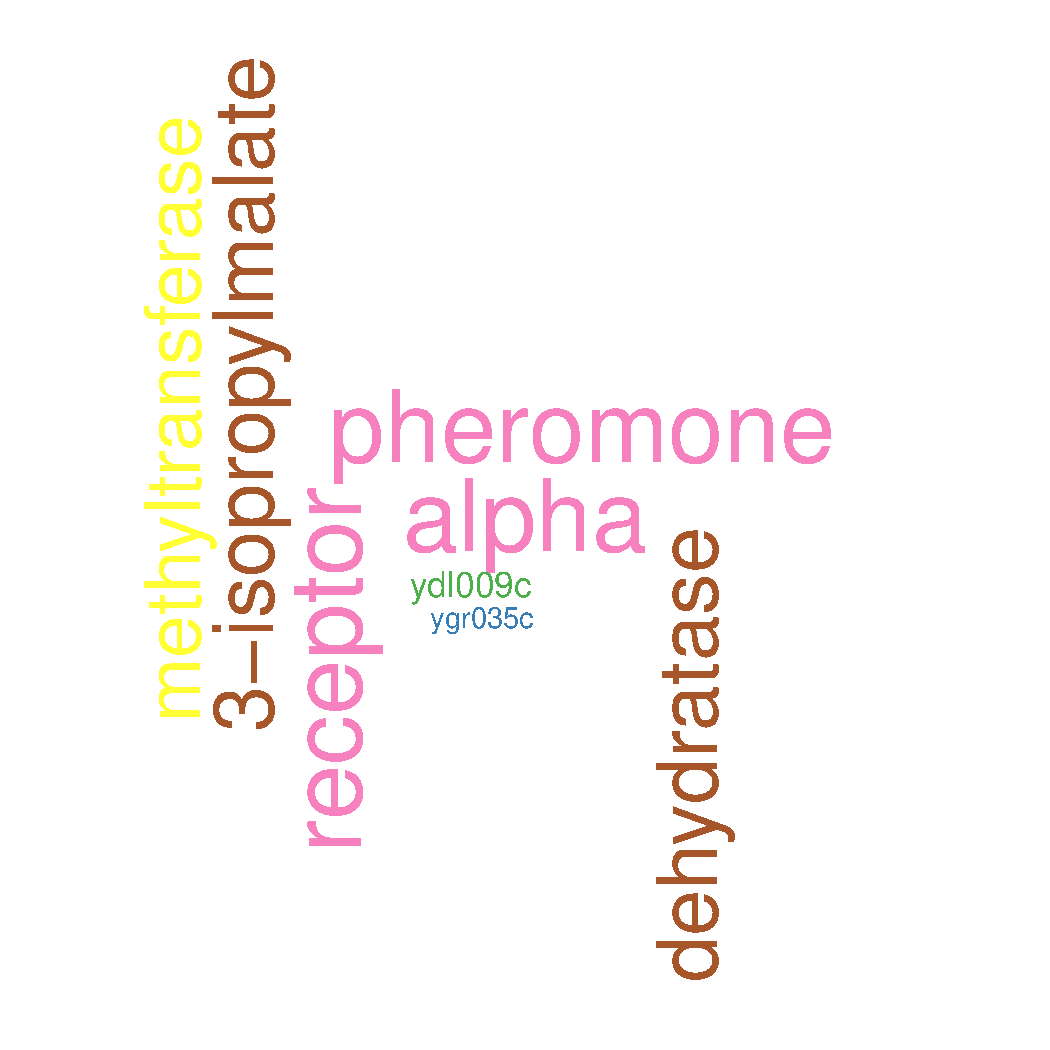
\includegraphics[width=\textwidth]{11_edgeR_wordcloud_cn2_down.pdf} % Replace with your image
        \caption{}
        \label{fig:wc_neg_edger_2}
    \end{subfigure}
    % Overall figure caption
    \caption{Results from the four experiments: (a) First experiment, (b) Second experiment, (c) Third experiment, (d) Fourth experiment.}
    \label{fig:wc_top_edger}
\end{figure}

\begin{figure}[H]
    \centering
    % Top-left subfigure
    \begin{subfigure}[b]{0.45\textwidth}
        \centering
        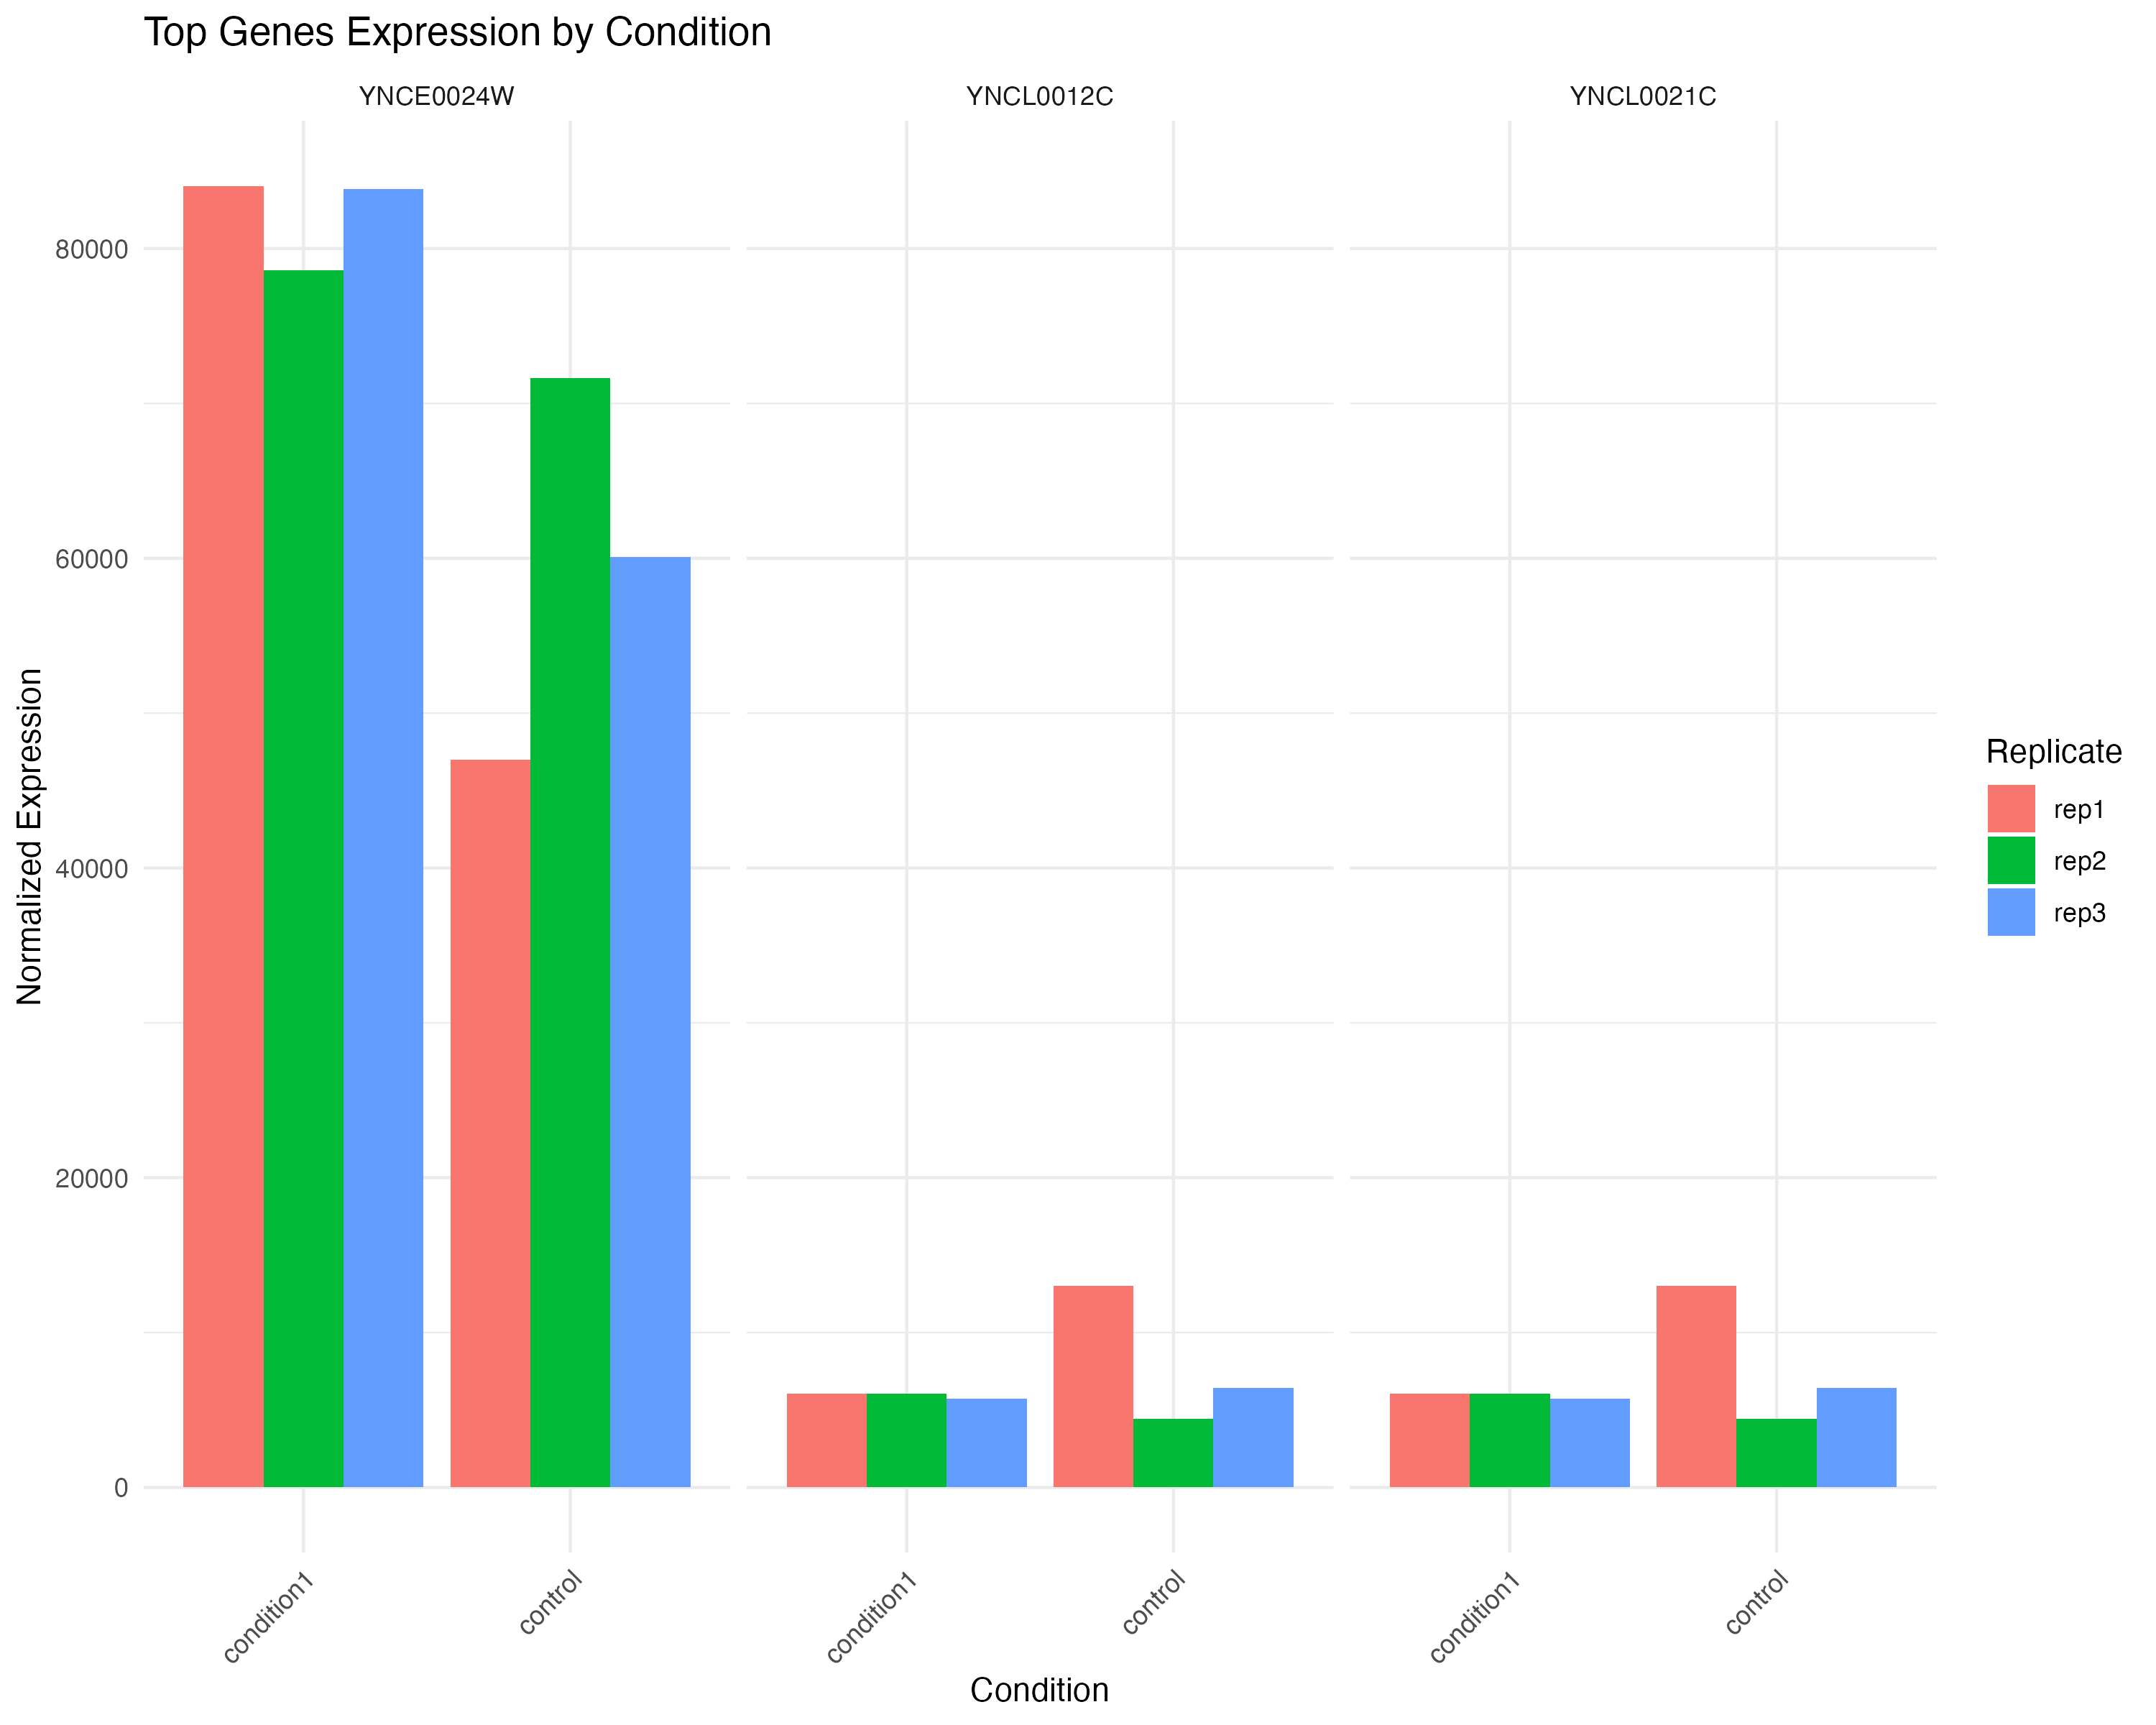
\includegraphics[width=\textwidth]{11_top_positive_genes_expression_by_condition1_limma.png} % Replace with your image
        \caption{}
        \label{fig:pos_limma_1}
    \end{subfigure}
    \hfill
    % Top-right subfigure
    \begin{subfigure}[b]{0.45\textwidth}
        \centering
        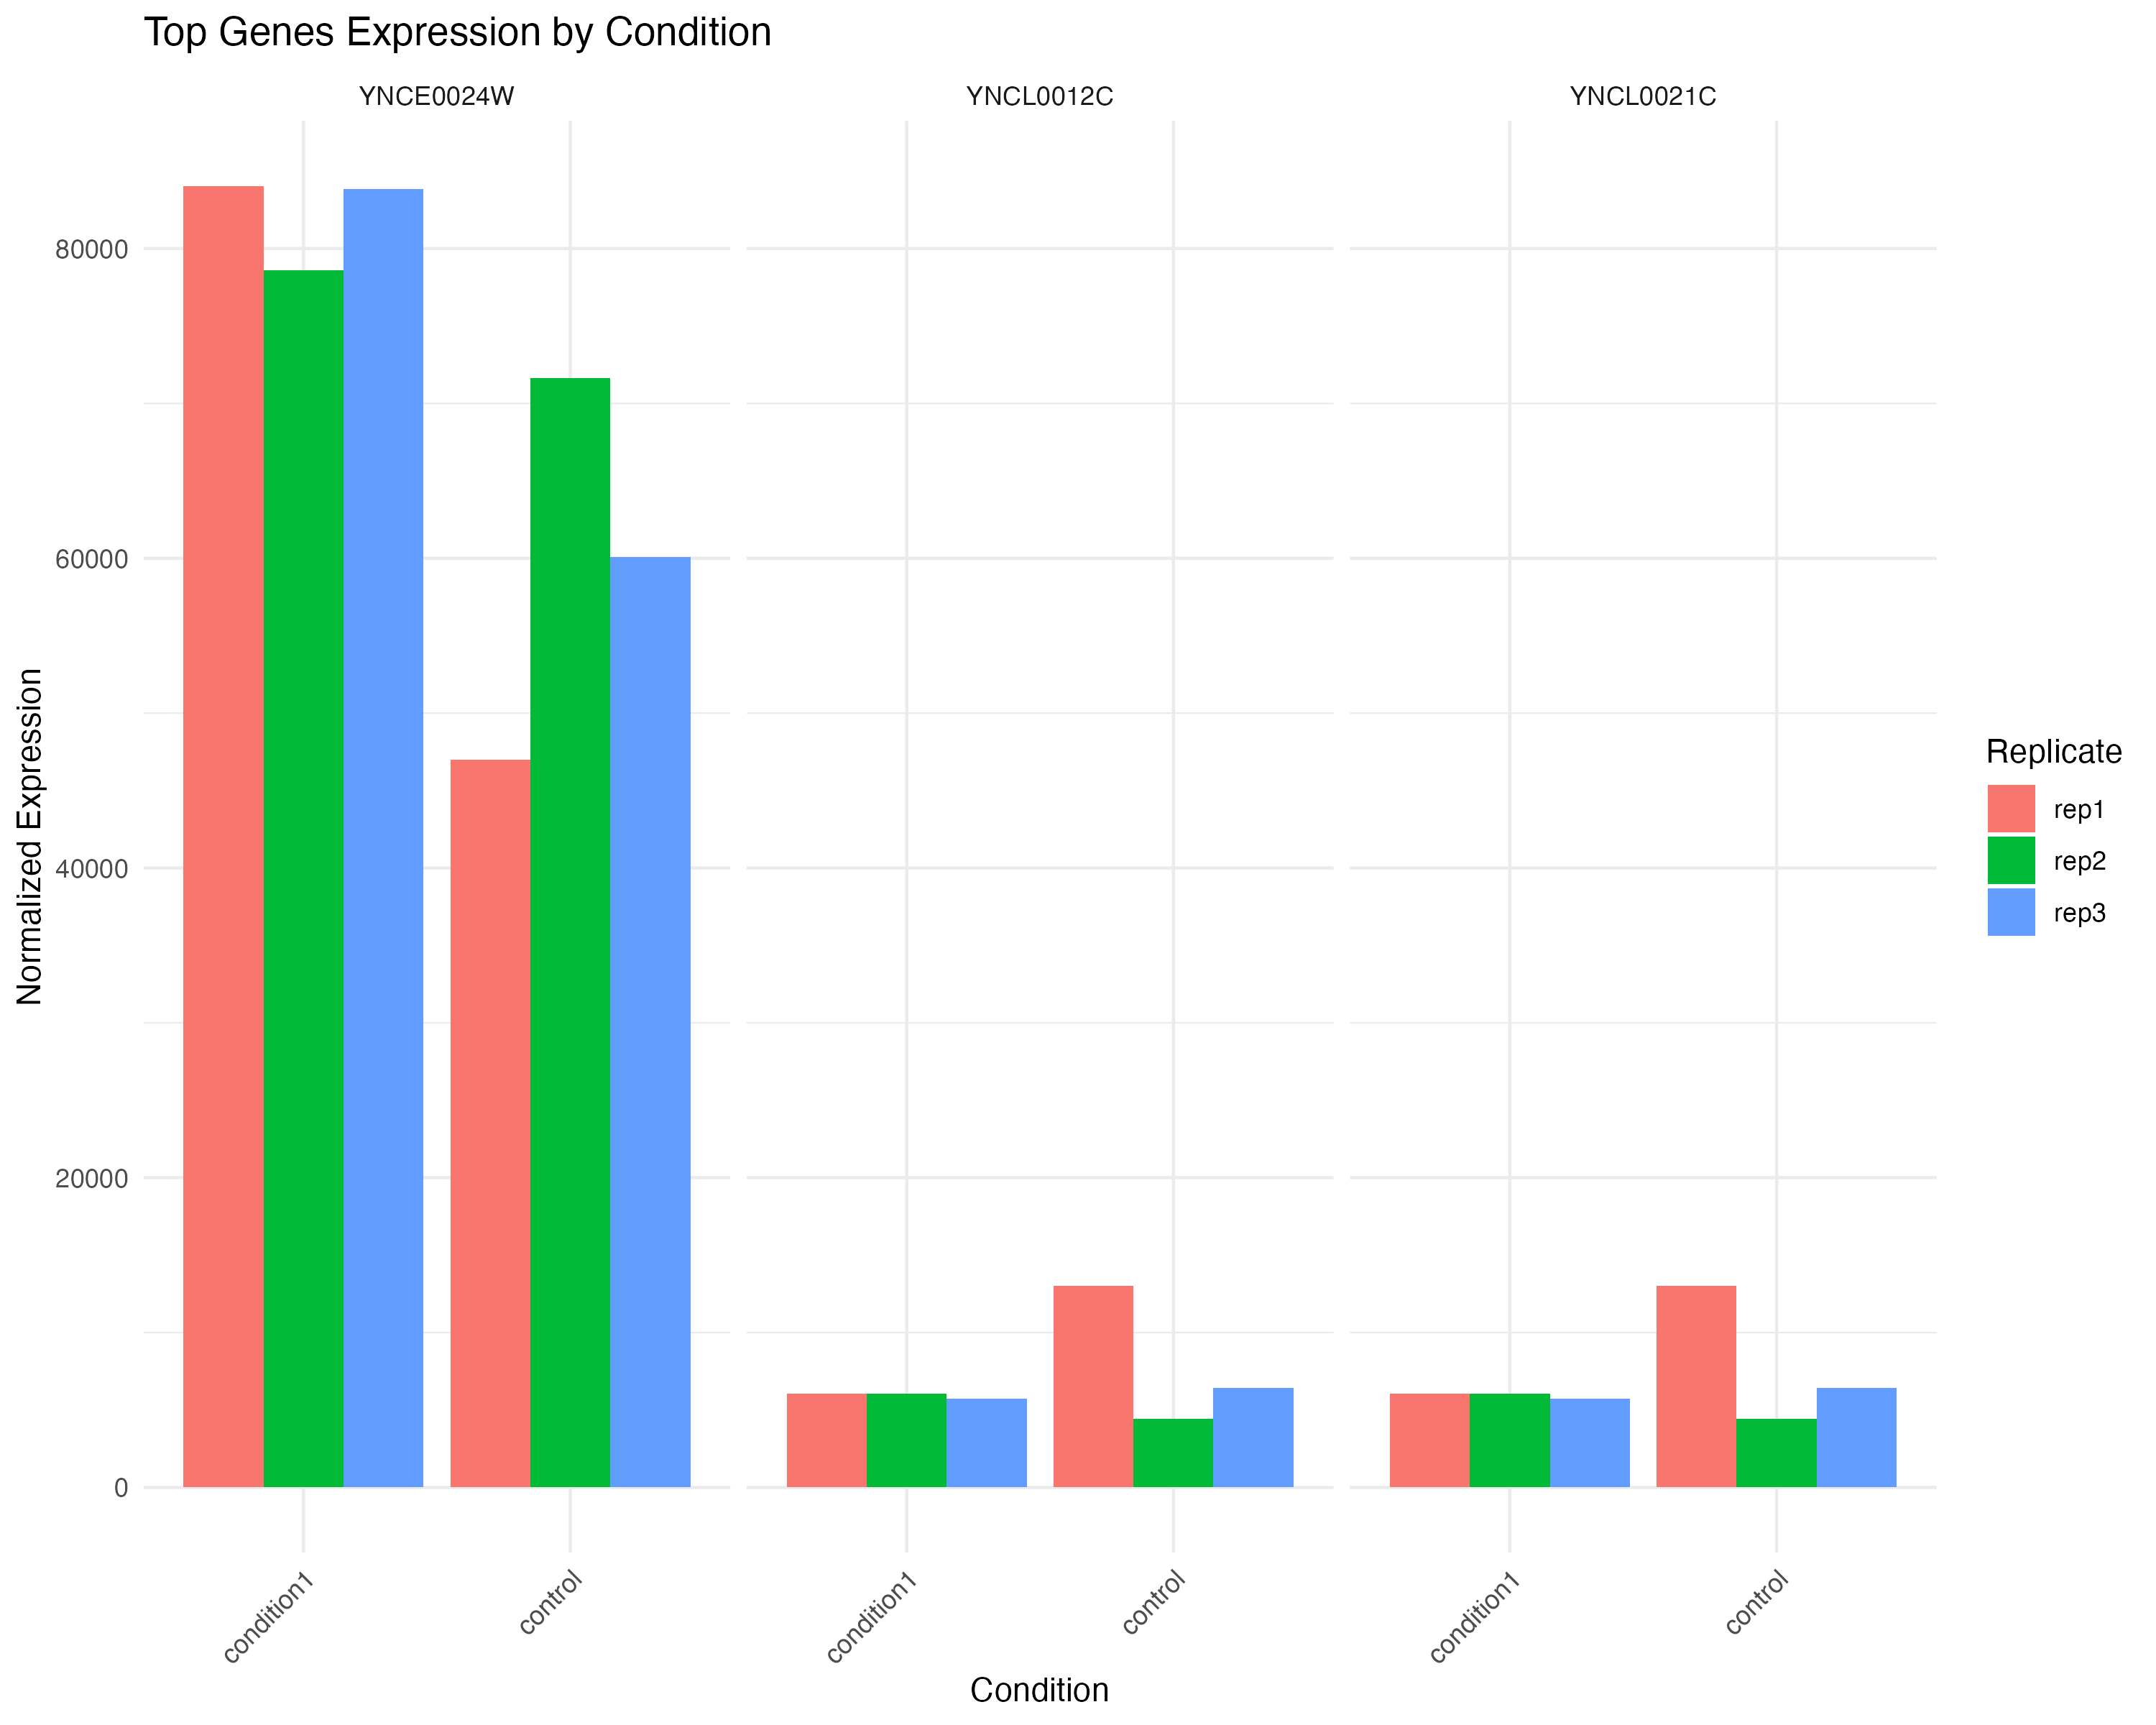
\includegraphics[width=\textwidth]{11_top_positive_genes_expression_by_condition2_limma.png} % Replace with your image
        \caption{}
        \label{fig:pos_limma_2}
    \end{subfigure}
    \vskip\baselineskip % Vertical space between rows
    % Bottom-left subfigure
    \begin{subfigure}[b]{0.45\textwidth}
        \centering
        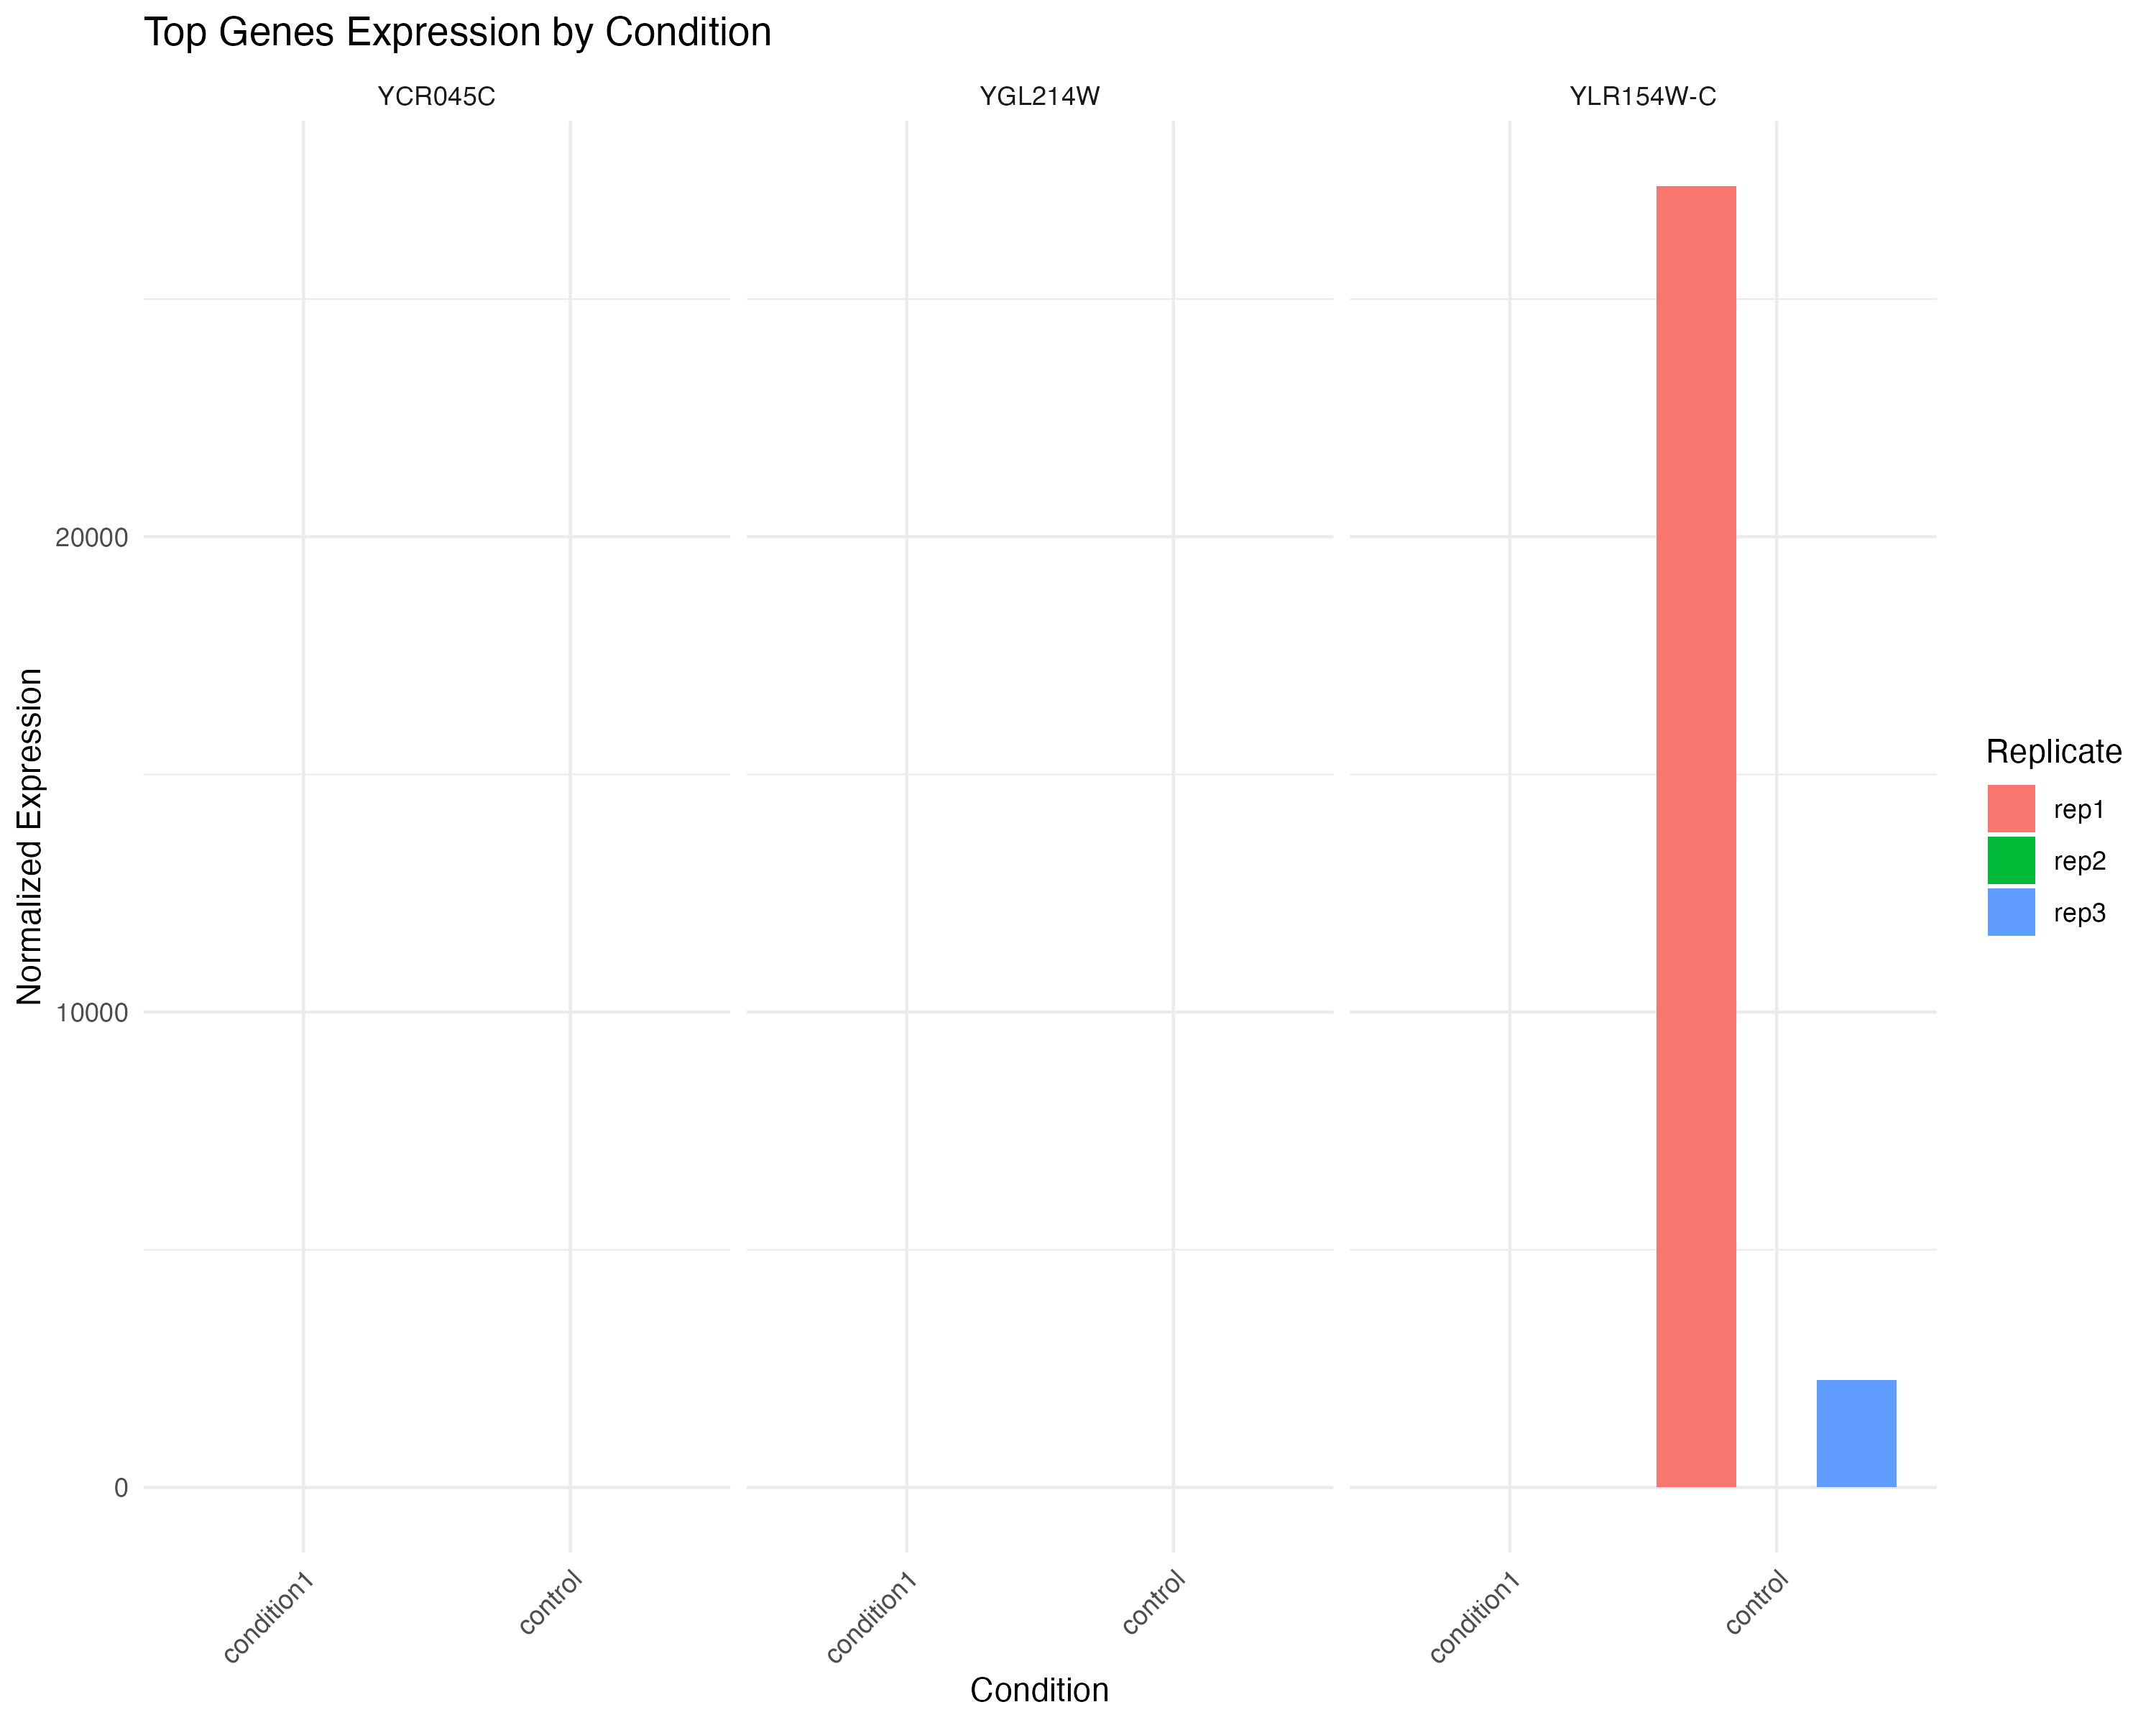
\includegraphics[width=\textwidth]{11_top_negative_genes_expression_by_condition1_limma.png} % Replace with your image
        \caption{}
        \label{fig:neg_limma_1}
    \end{subfigure}
    \hfill
    % Bottom-right subfigure
    \begin{subfigure}[b]{0.45\textwidth}
        \centering
        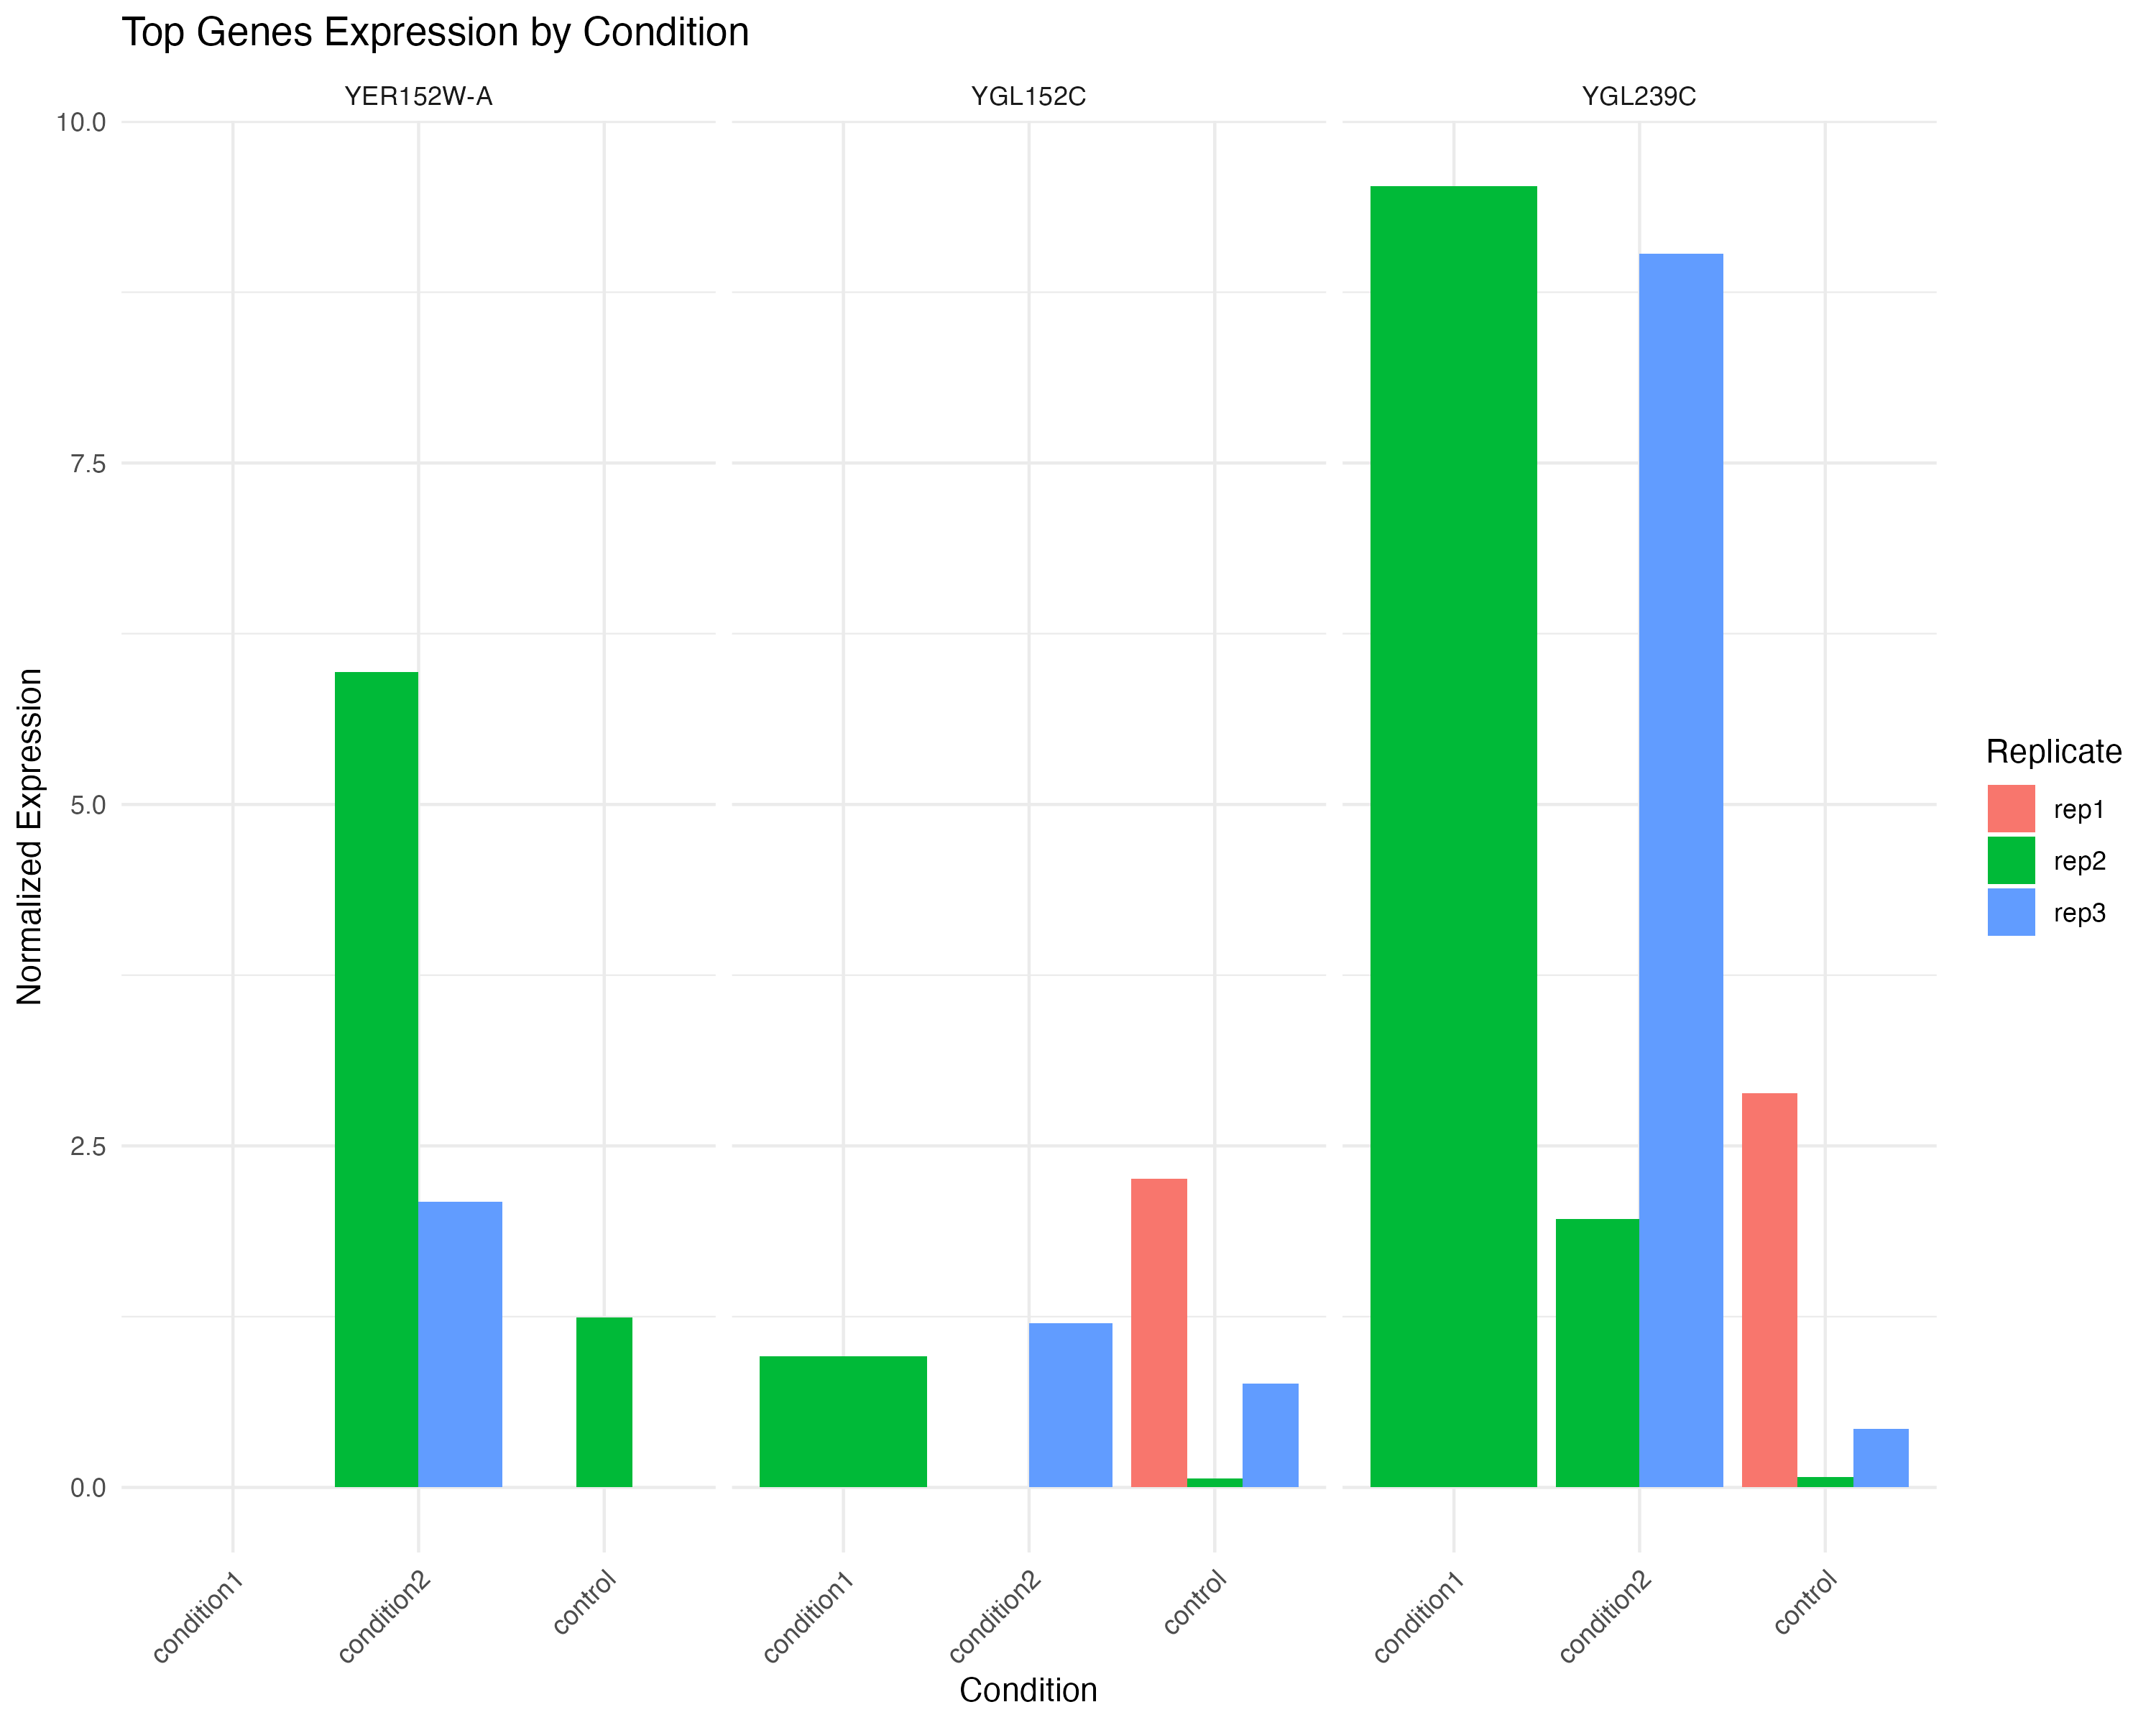
\includegraphics[width=\textwidth]{11_top_negative_genes_expression_by_condition2_limma.png} % Replace with your image
        \caption{}
        \label{fig:neg_limma_2}
    \end{subfigure}
    % Overall figure caption
    \caption{Results from the four experiments: (a) First experiment, (b) Second experiment, (c) Third experiment, (d) Fourth experiment.}
    \label{fig:top_limma}
\end{figure}

\begin{figure}[H]
    \centering
    % Top-left subfigure
    \begin{subfigure}[b]{0.45\textwidth}
        \centering
        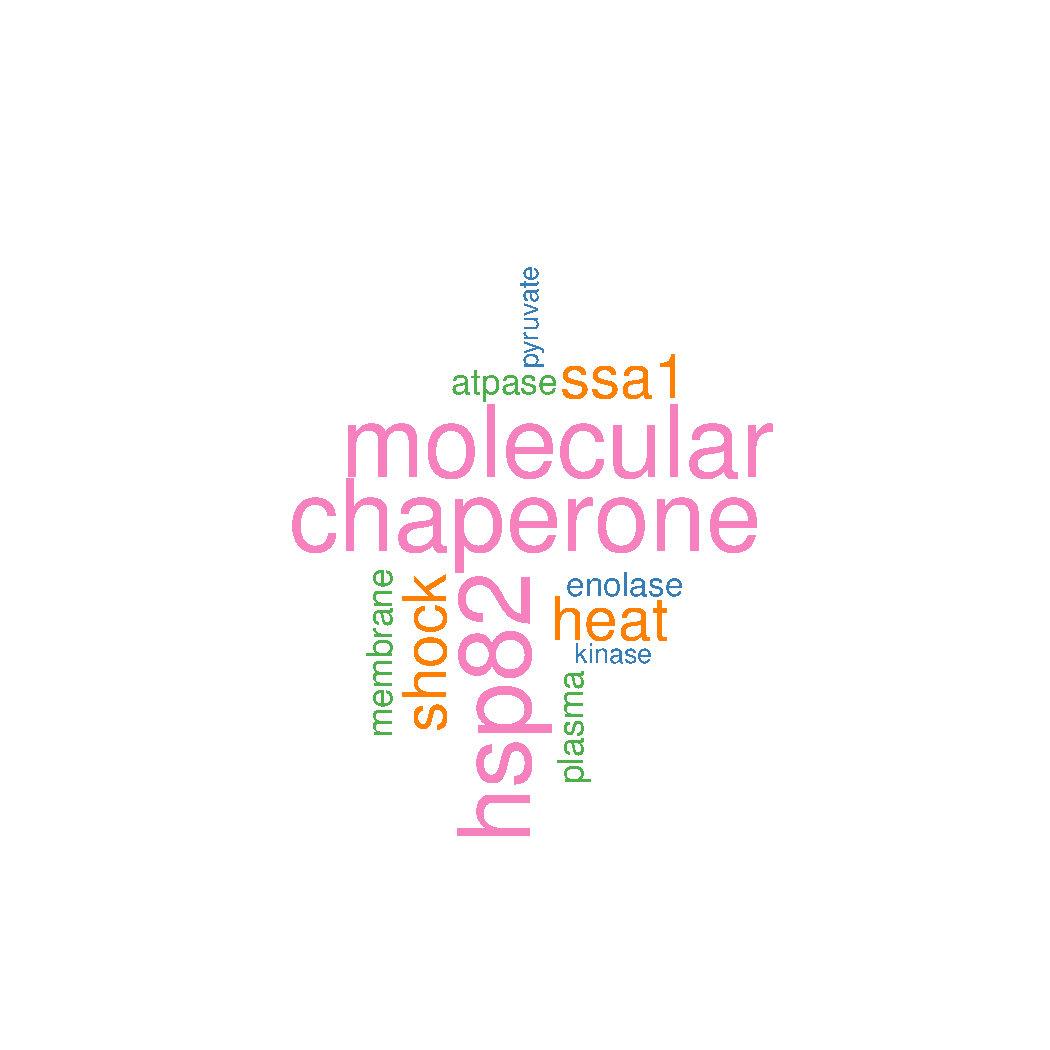
\includegraphics[width=\textwidth]{11_limma_wordcloud_cn1_up.pdf} % Replace with your image
        \caption{}
        \label{fig:wc_pos_limma_1}
    \end{subfigure}
    \hfill
    % Top-right subfigure
    \begin{subfigure}[b]{0.45\textwidth}
        \centering
        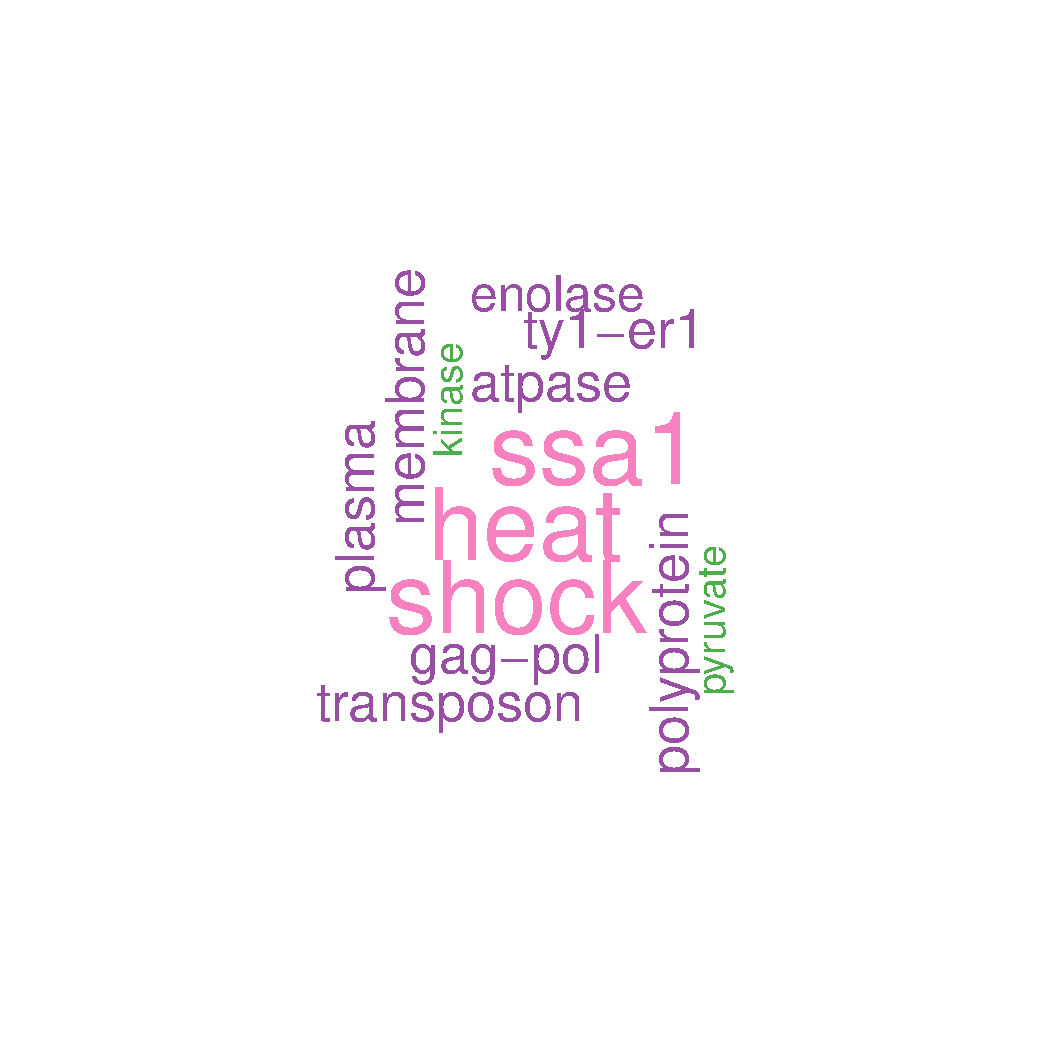
\includegraphics[width=\textwidth]{11_limma_wordcloud_cn2_up.pdf} % Replace with your image
        \caption{}
        \label{fig:wc_pos_limma_2}
    \end{subfigure}
    \vskip\baselineskip % Vertical space between rows
    % Bottom-left subfigure
    \begin{subfigure}[b]{0.45\textwidth}
        \centering
        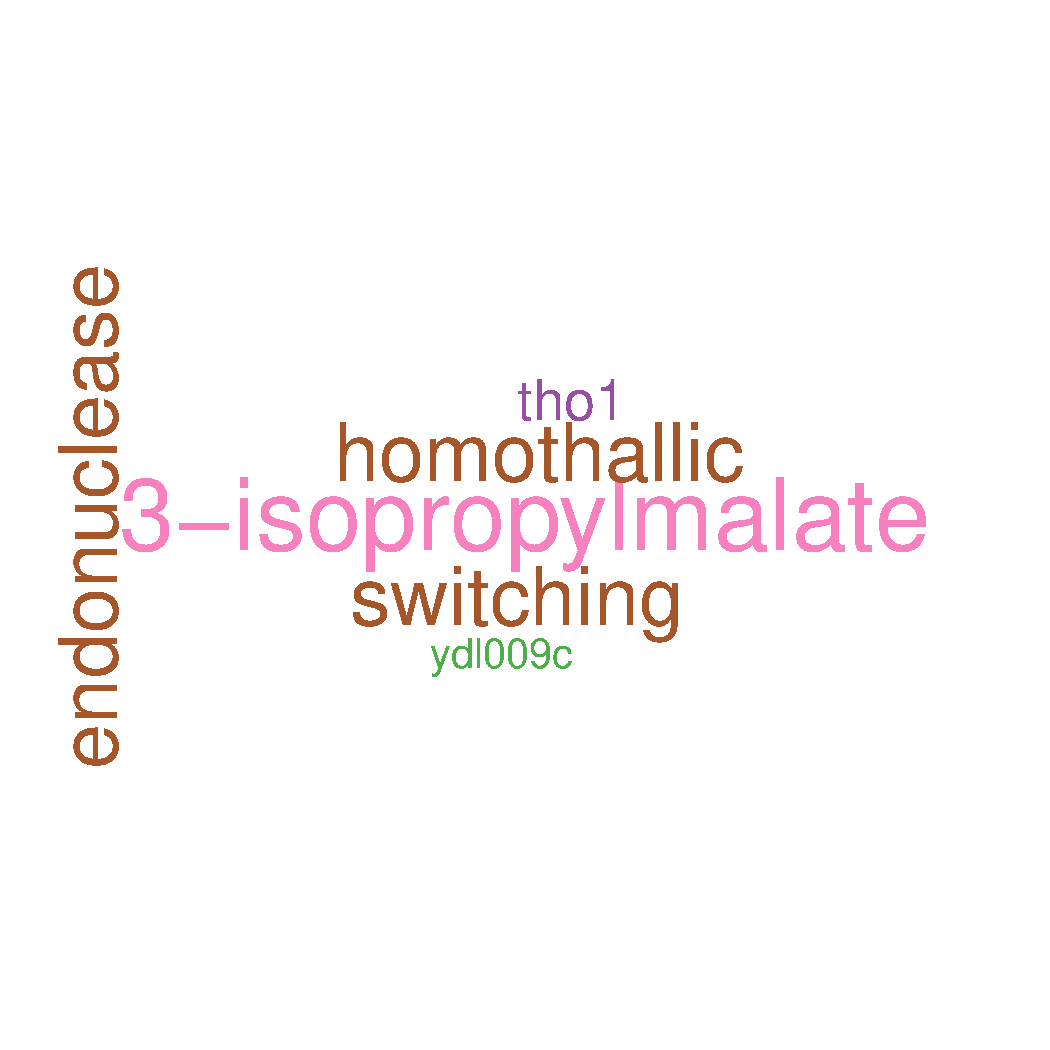
\includegraphics[width=\textwidth]{11_limma_wordcloud_cn1_down.pdf} % Replace with your image
        \caption{}
        \label{fig:wc_neg_limma_1}
    \end{subfigure}
    \hfill
    % Bottom-right subfigure
    \begin{subfigure}[b]{0.45\textwidth}
        \centering
        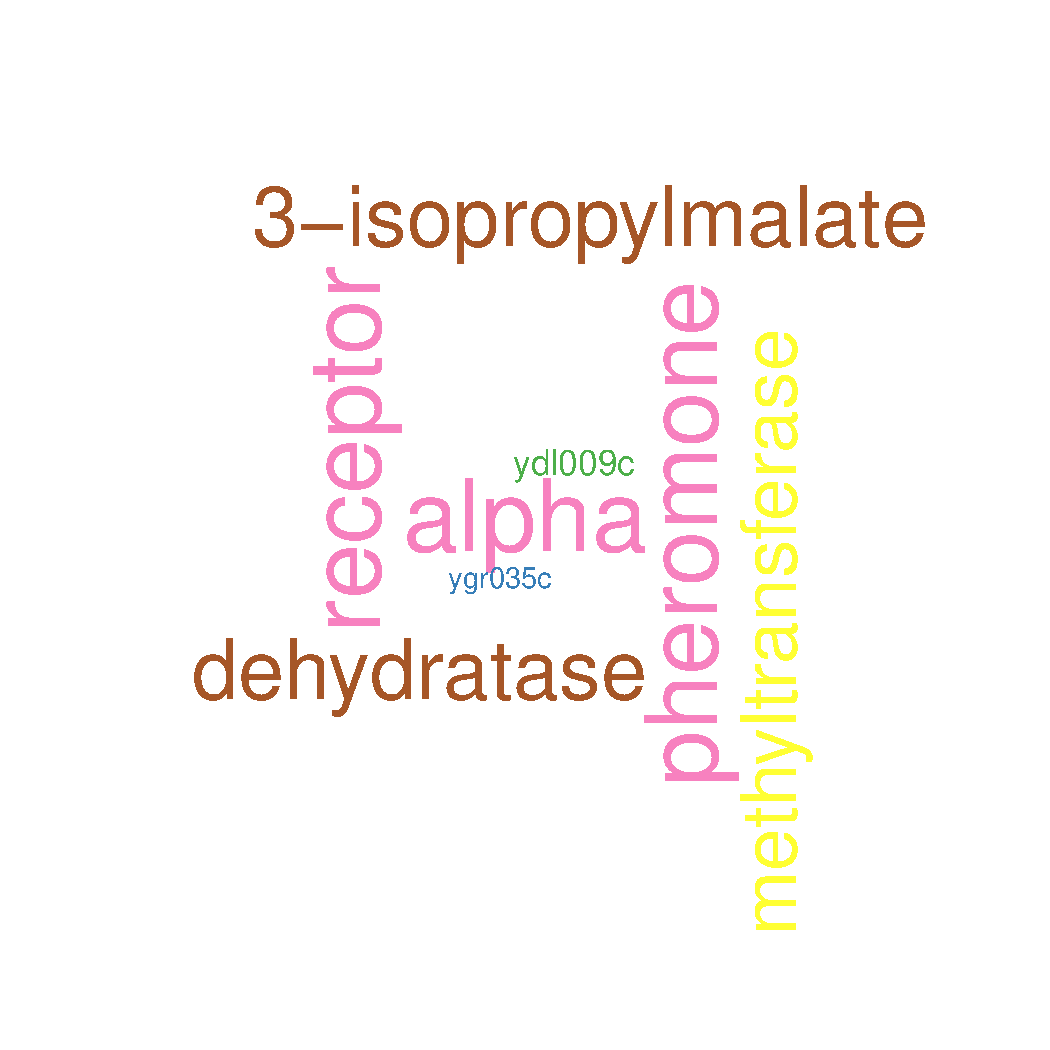
\includegraphics[width=\textwidth]{11_wordcloud_cn2_down.pdf} % Replace with your image
        \caption{}
        \label{fig:wc_neg_limma_2}
    \end{subfigure}
    % Overall figure caption
    \caption{Results from the four experiments: (a) First experiment, (b) Second experiment, (c) Third experiment, (d) Fourth experiment.}
    \label{fig:wc_top_limma}
\end{figure}


